%% DA6400 Programming Assignment 3 — Report
%% Compile with: pdflatex main.tex (run twice for cross-references)

\documentclass[11pt,a4paper]{article}

\usepackage[top=0.9in,bottom=0.9in,left=0.9in,right=0.9in]{geometry}
\usepackage{amsmath,amssymb}
\usepackage{graphicx}
\graphicspath{{figures/}}
\usepackage{booktabs}
\usepackage{multirow}
\usepackage{hyperref}
\usepackage[font=small,labelfont=bf]{caption}
\usepackage{subcaption}
\usepackage{float}
\usepackage{array}
\usepackage{xcolor}
\usepackage[shortlabels]{enumitem}
\usepackage{microtype}
\usepackage{parskip}
\usepackage{appendix}

\setlength{\parskip}{3pt}
\setlength{\parindent}{0pt}
\setlist{noitemsep, topsep=2pt}

\hypersetup{colorlinks=true, linkcolor=blue, urlcolor=blue}

\title{\large\textbf{DA6400 : Reinforcement Learning (January--May 2026)\\
Programming Assignment 3 Submission}}

\author{
\textbf{Ananya Lakshmi Ravi}$^{*}$ \quad
\textbf{S Shriprasad}$^{*}$ \\[4pt]
\small NS26Z145 \qquad DA25E054 \\[2pt]
\small $^{*}$Equal Contribution
}
\date{}

\begin{document}
\maketitle

\vspace{-10pt}
\begin{center}
  \href{<PASTE_SOURCE_CODE_LINK_HERE>}{{\color{blue}$\triangleright$~Source Code}}
\end{center}
\vspace{-6pt}

% ============================================================
% SECTION 2.1: PENDULUM
% ============================================================
\section{Section 2.1: Pendulum}

\subsection{Environment and Reward Design}

We modify \texttt{Pendulum-v1} to stabilize at a target angle $\theta_{\text{target}}$. The observation is $s_t = (\cos\theta_t, \sin\theta_t, \dot\theta_t)$ and the action $u_t$ is the applied torque. Episodes are fixed-length (1000 steps) with no terminal state. We designed the reward:
\begin{equation}
r_t = -\text{reward\_scale}\left(w_\theta e_t^2 + w_\omega \dot\theta_t^2 + w_u u_t^2\right), \quad e_t = \mathrm{wrap}(\theta_t - \theta_{\text{target}}),
\label{eq:pendulum_reward}
\end{equation}
with $w_\theta=1.0$, $w_\omega=0.1$, $w_u=0.001$. The reward penalizes three quantities:
\begin{itemize}
    \item $w_\theta e_t^2$: squared wrapped angle error --- makes $\theta_{\text{target}}$ the unique optimum.
    \item $w_\omega \dot\theta_t^2$: angular velocity --- prevents swinging through the target; encourages stabilization.
    \item $w_u u_t^2$: torque --- discourages aggressive control, promotes smooth actuation.
\end{itemize}
The reward is dense (non-zero at every step). The target angle enters only via $e_t$, so the reward structure is identical across all targets.

We implemented SAC with tanh-squashed Gaussian policy, clipped double Q-learning, target networks, reparameterized actor updates, Adam optimizer, and automatic entropy temperature tuning (unless specified otherwise). All curves plot mean return vs.\ environment timesteps with 95\% CI over 15 seeds, using 20 offline evaluation episodes every 10K steps.

\subsection{SAC Across Target Angles}

Figure~\ref{fig:pendulum_auto_main} shows auto-$\alpha$ SAC for $\theta_{\text{target}} \in \{0,-10,30,-60,90,-90,120,-150\}^\circ$.

\begin{figure}[H]
\centering
\begin{subfigure}[t]{0.49\textwidth}
    \centering
    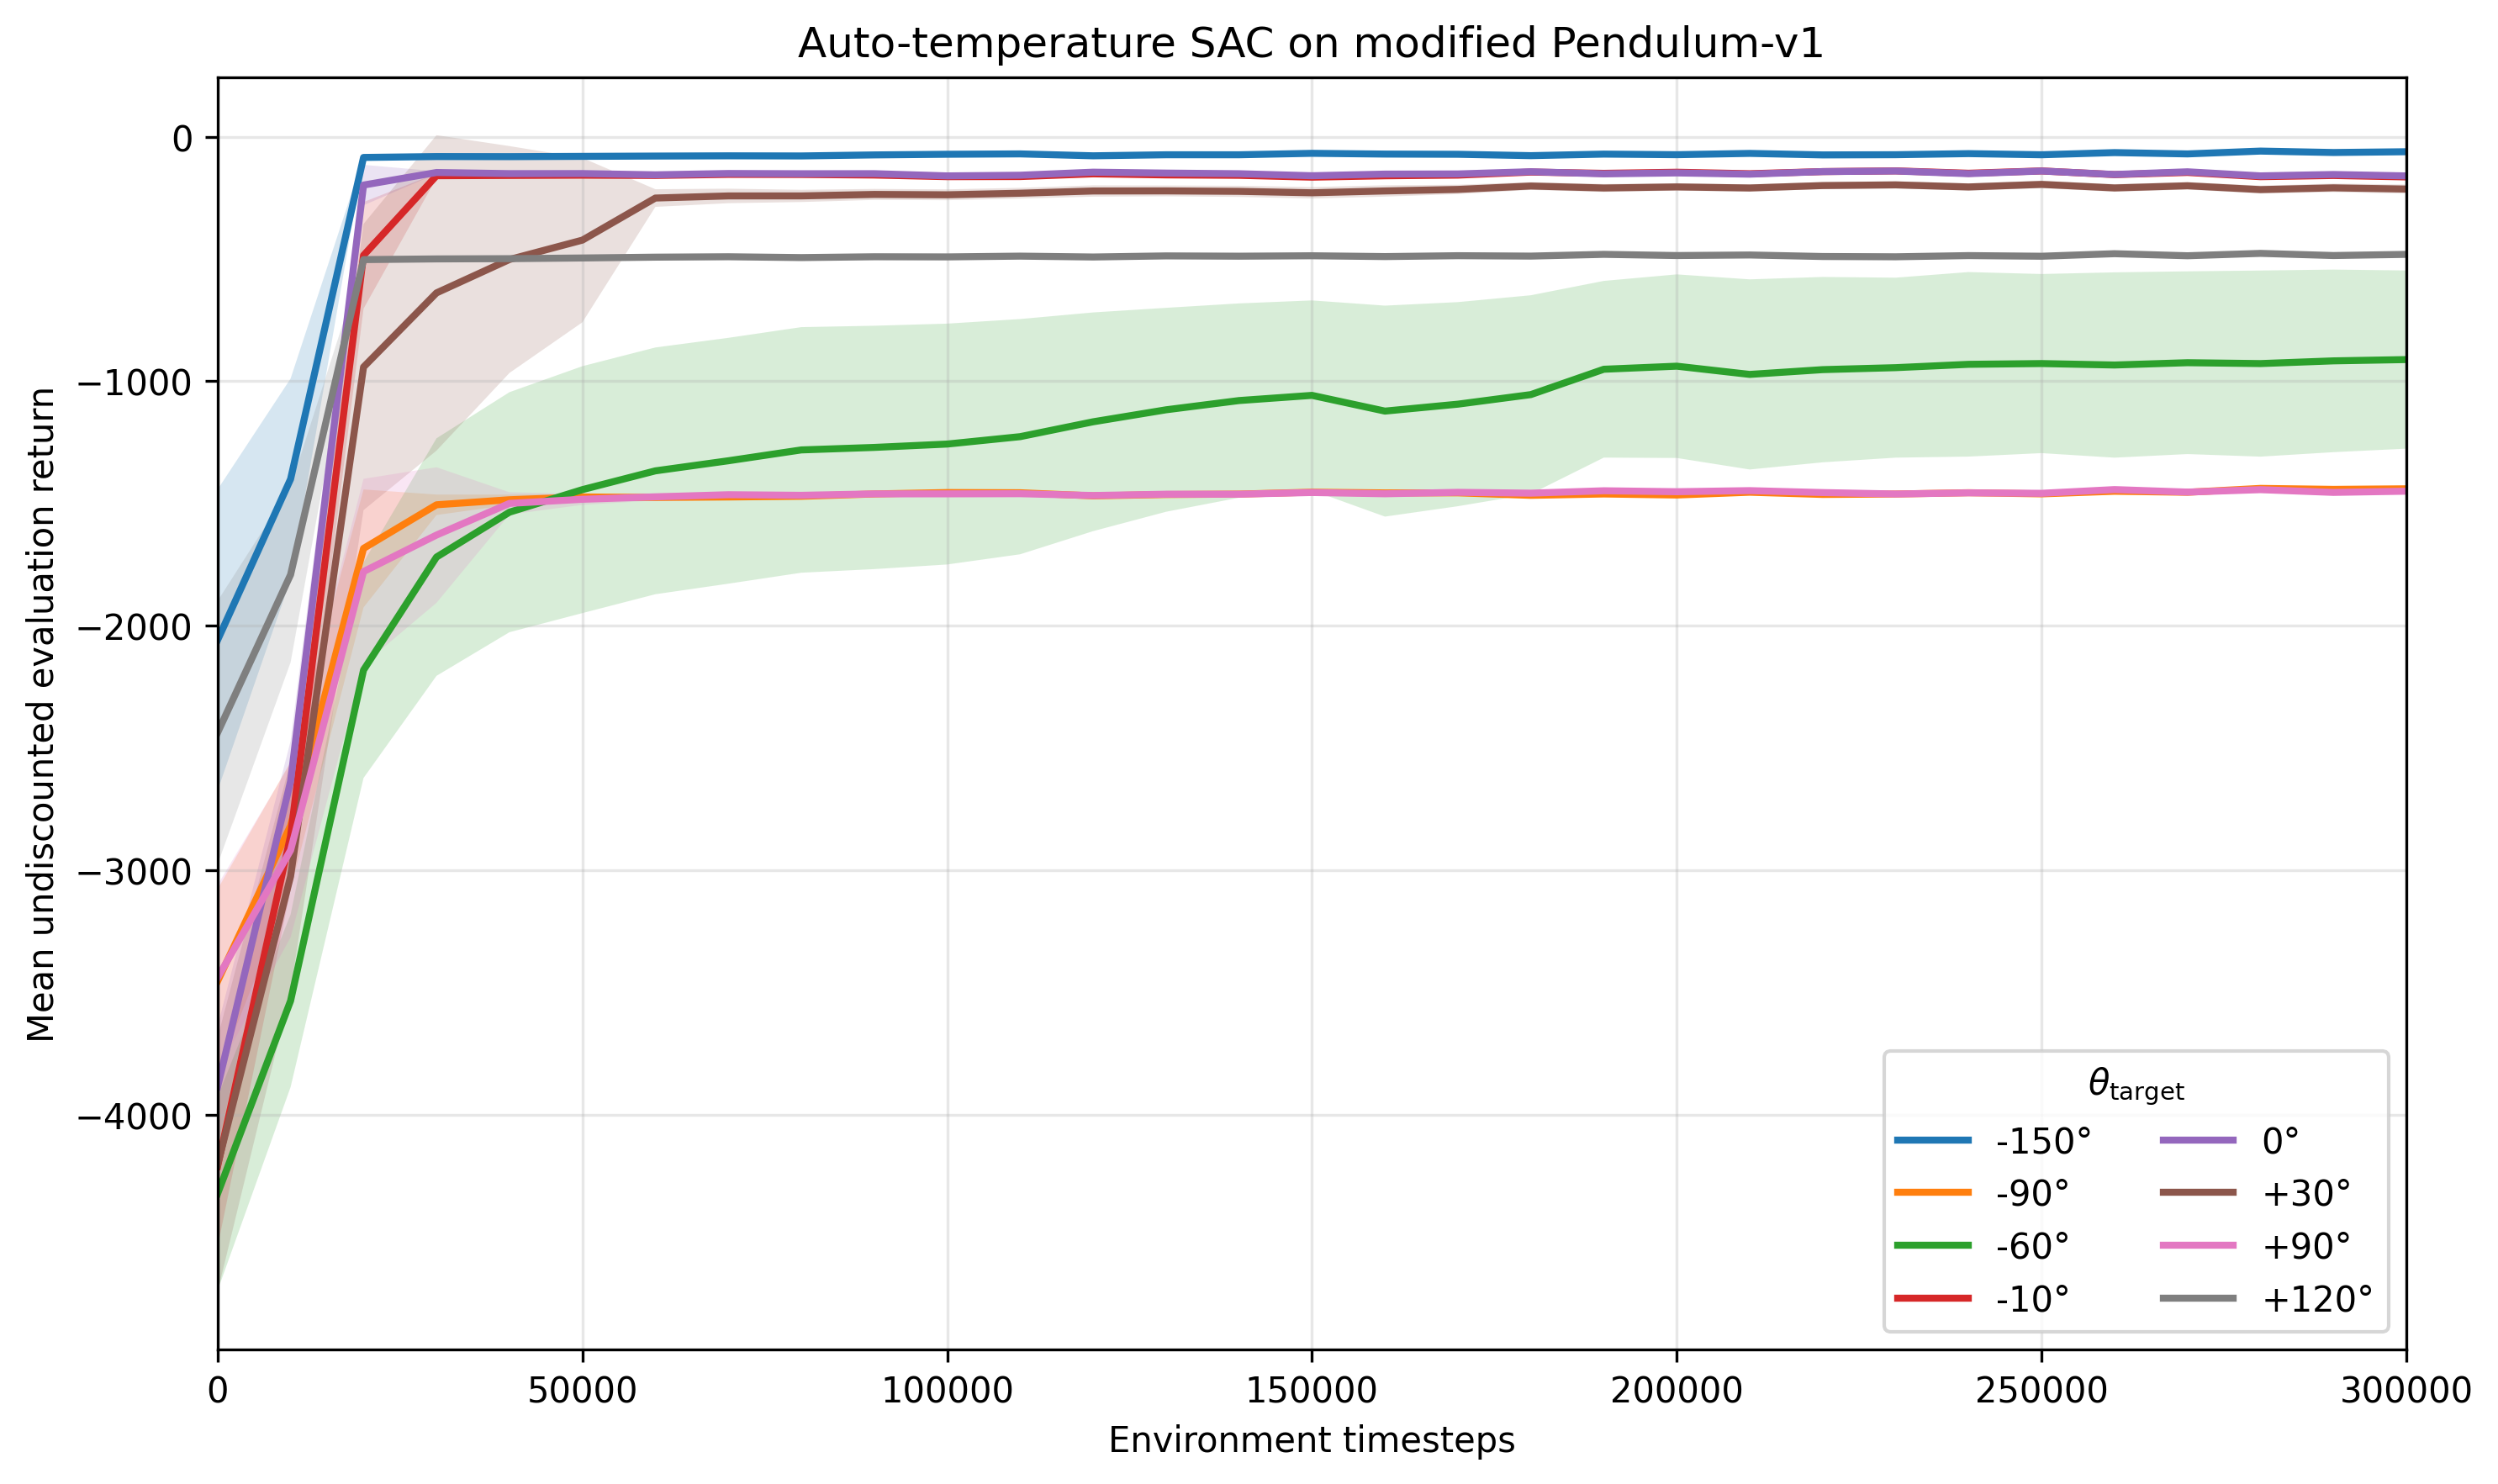
\includegraphics[width=\linewidth]{P1_auto_all_targets_eval_return_mean.png}
    \caption{Mean evaluation return.}
\end{subfigure}\hfill
\begin{subfigure}[t]{0.49\textwidth}
    \centering
    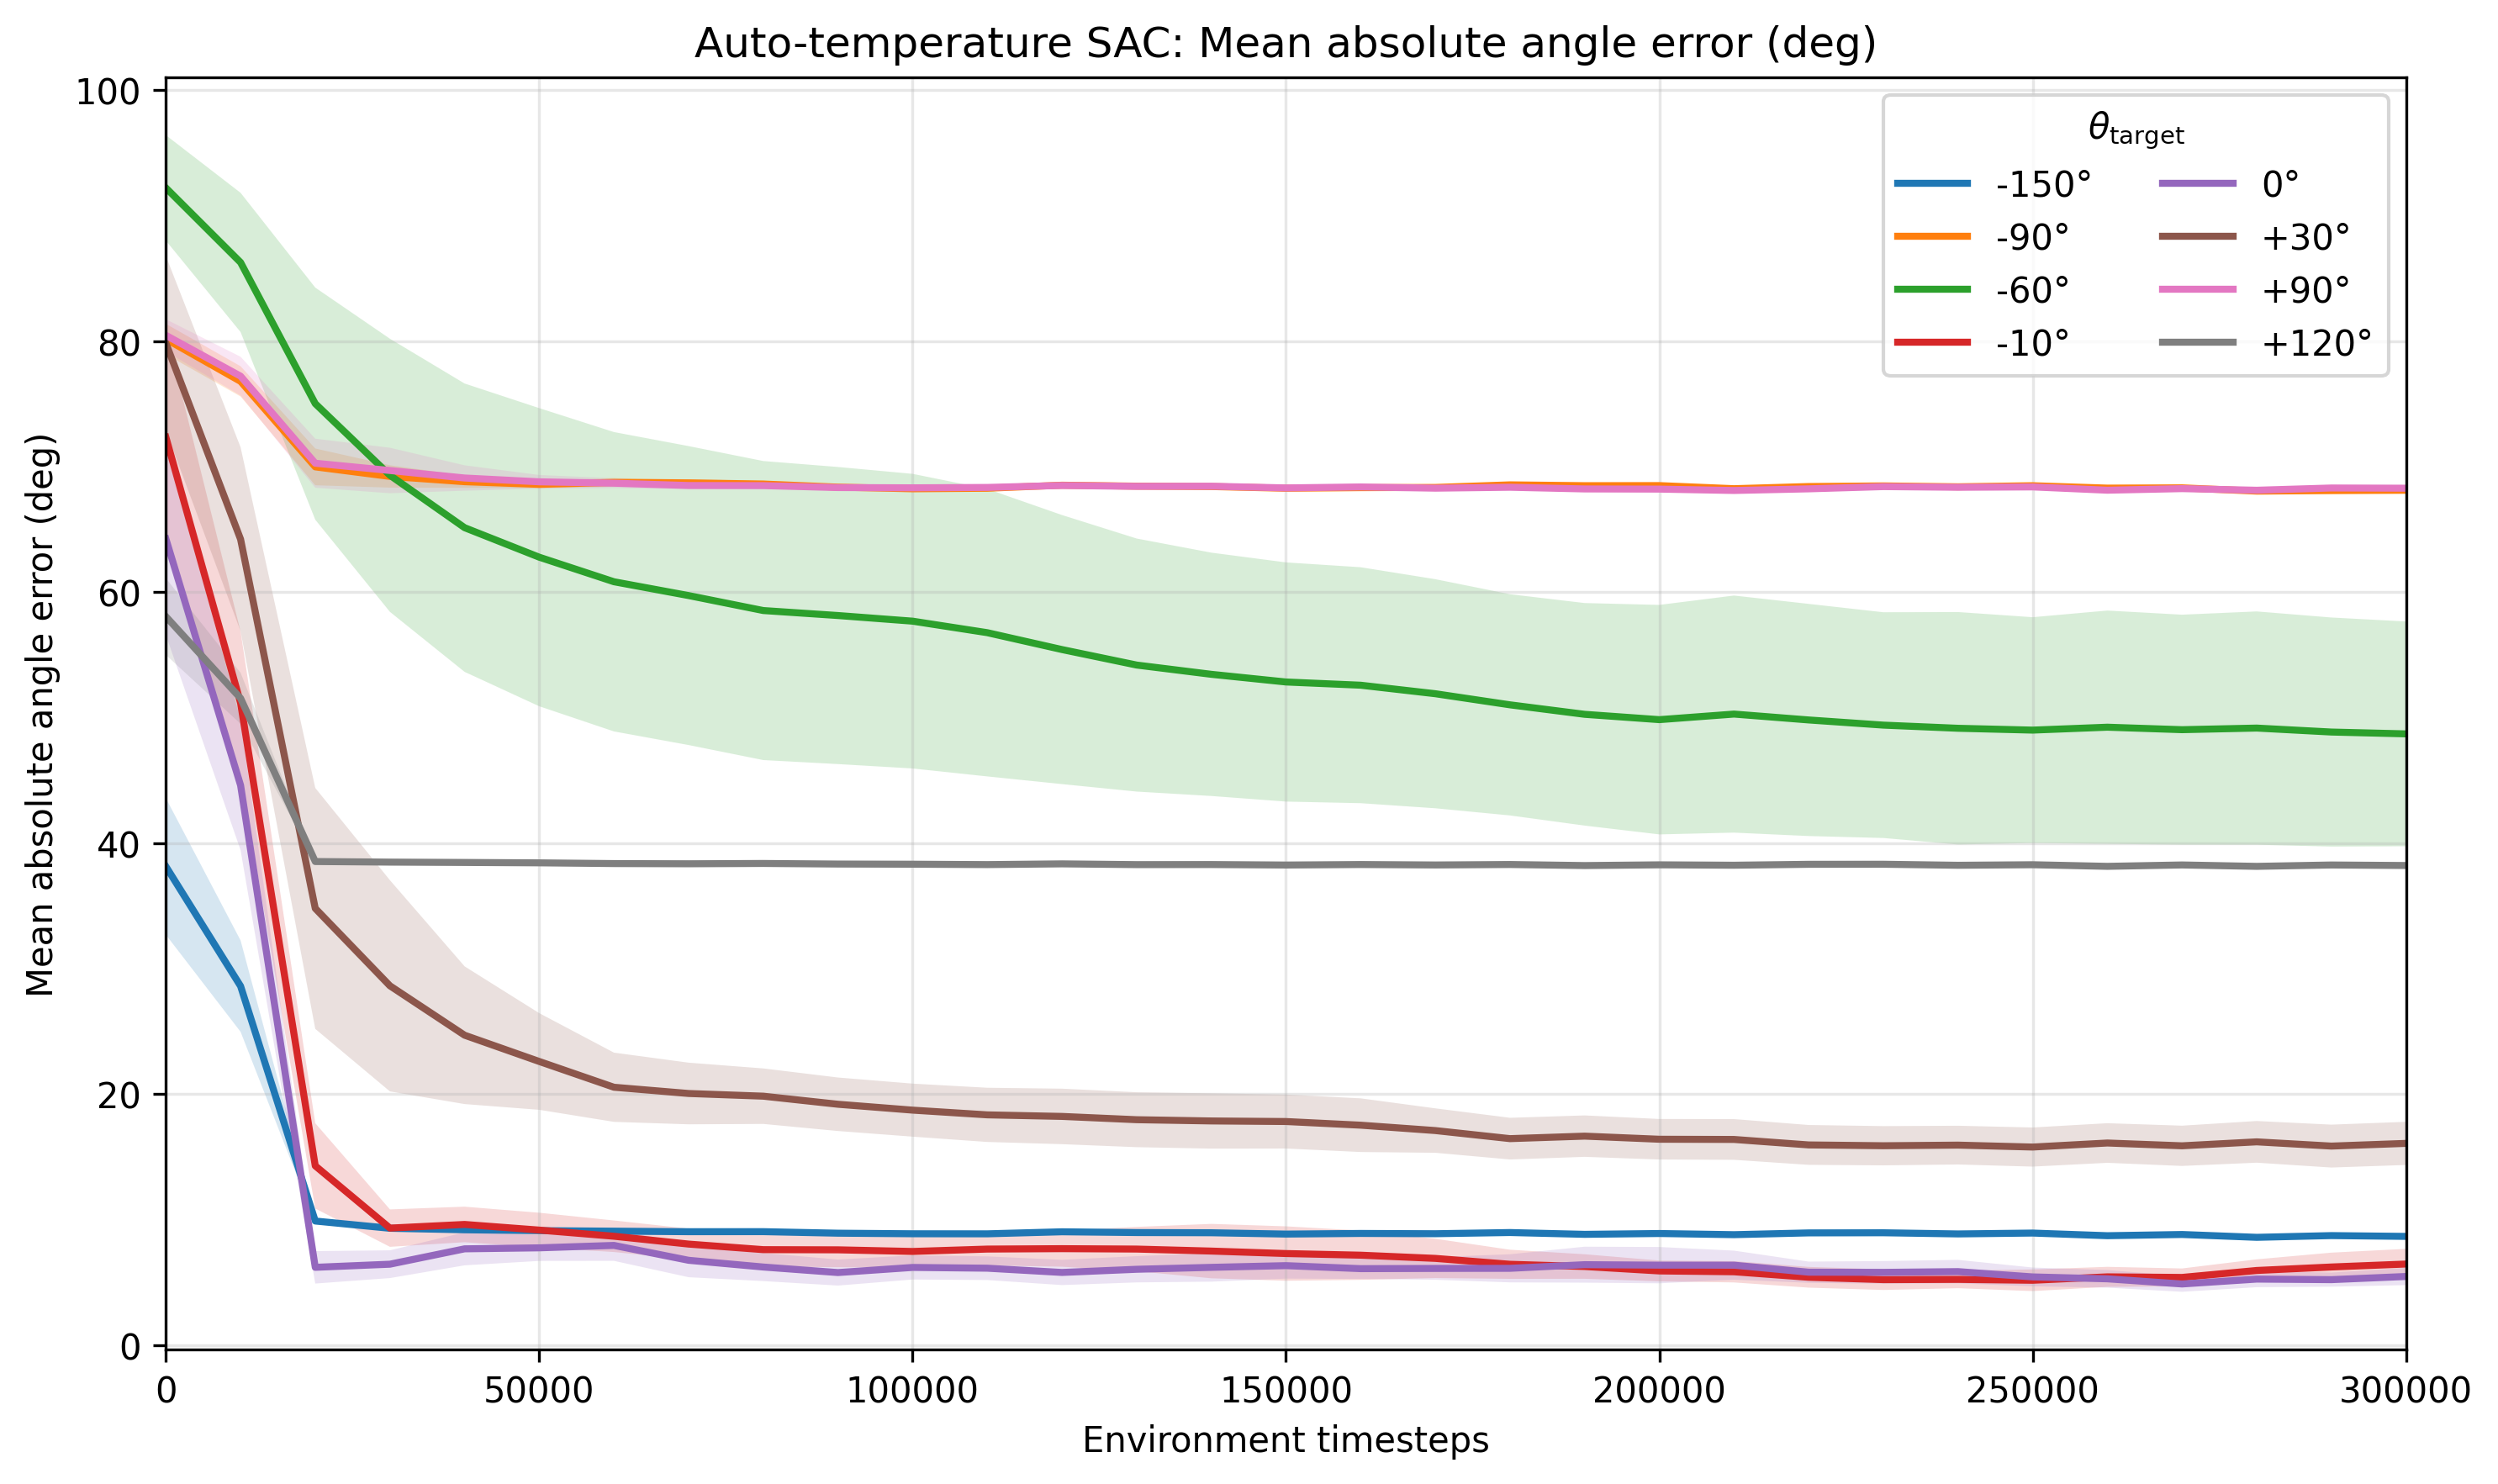
\includegraphics[width=\linewidth]{P1b_auto_all_targets_angle_error.png}
    \caption{Mean absolute angle error.}
\end{subfigure}
\caption{Auto-$\alpha$ SAC across target angles (mean $\pm$ 95\% CI).}
\label{fig:pendulum_auto_main}
\end{figure}

\textbf{Easy targets} ($0^\circ$, $-10^\circ$, $-150^\circ$) converge to low angle error ($<9^\circ$) and high target occupancy ($>0.95$). These targets require little or no sustained torque against gravity.

\textbf{Hard targets} ($\pm90^\circ$, $-60^\circ$, $120^\circ$) do not converge to the exact target angle. The reason is the default torque bound. In Gymnasium's Pendulum-v1 ($m=1$, $l=1$, $g=10$), the approximate static holding torque for a target angle is
\[
|u_{\text{hold}}| = \frac{mgl}{2}|\sin\theta_{\text{target}}| = 5|\sin\theta_{\text{target}}|.
\]
The default action bound is $|u|\leq 2$. For targets such as $\pm90^\circ$ ($|u_{\text{hold}}|=5.0$), $-60^\circ$ and $120^\circ$ ($|u_{\text{hold}}|=4.33$), the required holding torque exceeds the available range. The policy still learns useful behavior---it damps oscillations and reduces angular velocity---but it stabilizes at a compromise angle closer to the natural equilibrium rather than exactly at the target.

The $-60^\circ$ target shows high seed-to-seed variability ($-903.54 \pm 368.75$): some seeds discover a viable control strategy while others settle into a low-effort equilibrium. Its mean curve should be interpreted together with the wide confidence interval.

\textbf{Target occupancy} is the fraction of evaluation timesteps for which the wrapped angle error lies within a $10^\circ$ tolerance.

\begin{table}[H]
\centering
\caption{Final auto-$\alpha$ SAC results across target angles.}
\label{tab:pendulum_auto_final}
\resizebox{\textwidth}{!}{
\begin{tabular}{rrrrr}
\toprule
$\theta_{\text{target}}$ & Final Return & Angle Error (deg) & Target Occupancy & Mean Sq.\ Torque \\
\midrule
$-150^\circ$ & $-72.79 \pm 3.04$ & $8.94$ & $0.971$ & $3.563$ \\
$-90^\circ$  & $-1449.92 \pm 6.81$ & $68.23$ & $0.0007$ & $3.512$ \\
$-60^\circ$  & $-903.54 \pm 368.75$ & $48.39$ & $0.002$ & $2.979$ \\
$-10^\circ$  & $-156.64 \pm 7.31$ & $6.37$ & $0.958$ & $0.919$ \\
$0^\circ$    & $-153.08 \pm 7.00$ & $5.13$ & $0.965$ & $0.209$ \\
$30^\circ$   & $-206.43 \pm 20.26$ & $15.76$ & $0.130$ & $2.131$ \\
$90^\circ$   & $-1468.75 \pm 9.92$ & $68.56$ & $0.0004$ & $3.464$ \\
$120^\circ$  & $-496.51 \pm 2.00$ & $38.39$ & $0.003$ & $3.618$ \\
\bottomrule
\end{tabular}}
\end{table}

\subsection{Optimal Behavior}

The optimal behavior has \textbf{two aspects}:
\begin{enumerate}
    \item \textbf{Reaching:} from the random initial state, move the pendulum toward $\theta_{\text{target}}$. Depending on the target, this may require one or more swings to build momentum.
    \item \textbf{Stabilization:} once near the target, maintain low wrapped angle error and low angular velocity for the remainder of the 1000-step episode. A policy that merely passes through the target without staying is suboptimal.
\end{enumerate}

Return alone does not distinguish these aspects. A policy can achieve low angular velocity yet stabilize at the wrong angle. We therefore also examine angle error, target occupancy, angular velocity, and torque (Appendix~\ref{app:pendulum_diag}). For easy targets, the policy achieves both reaching and stabilization. For hard targets, the policy often damps oscillations effectively but stabilizes at a compromise angle, because exact target holding requires more torque than the default action bound allows.

We ran a diagnostic with wider torque $[-6,6]$ for $-60^\circ$, which achieved near-perfect tracking ($2$--$3^\circ$ error, occupancy $0.98$). This strongly supports the interpretation that the default $-60^\circ$ difficulty is mainly due to torque-limit and reward-tradeoff constraints, rather than SAC being unable to learn useful control (Appendix~\ref{app:torque_diag}).

\begin{figure}[H]
\centering
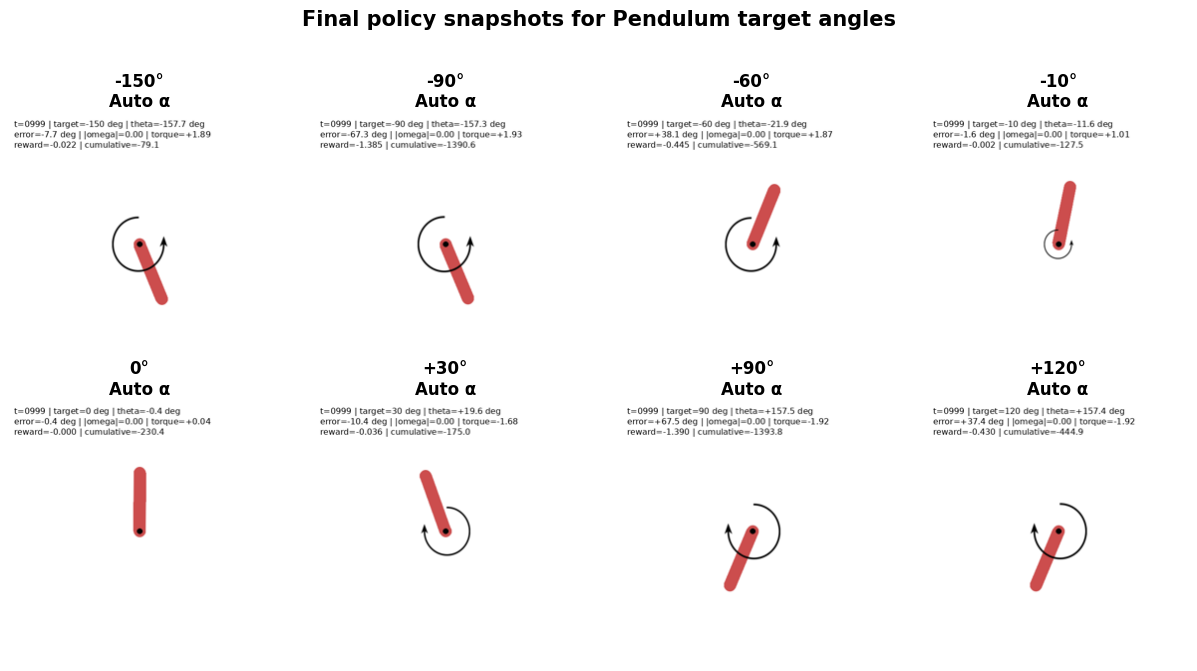
\includegraphics[width=0.92\textwidth, height=0.28\textheight, keepaspectratio]{pendulum_angles.png}
\caption{Final policy snapshots at $t=999$ for all target angles (auto-$\alpha$). Easy targets ($0^\circ$, $-10^\circ$, $-150^\circ$) show near-zero angle error. Hard targets ($\pm90^\circ$, $120^\circ$) stabilize at a compromise angle due to torque constraints. Note that all policies achieve $|\dot\theta|=0$ (successful damping), but only feasible targets achieve low angle error.}
\label{fig:pendulum_snapshots}
\end{figure}

\subsection{Manual vs.\ Automatic $\alpha$}

We searched $\alpha \in \{0.01, 0.03, 0.05, 0.1, 0.2, 0.5\}$ for $\theta \in \{-60, 90, 120, -150\}^\circ$. Selected: $\alpha_{\text{mnl}}=0.03$ for $-60^\circ$; $\alpha_{\text{mnl}}=0.01$ for $90^\circ$, $120^\circ$, and $-150^\circ$. This selection required $4 \times 6 \times 3 = 72$ pilot runs (4~targets, 6~alpha values, 3~tuning seeds) before the final comparison, making manual tuning significantly more expensive than automatic tuning.

\begin{figure}[H]
\centering
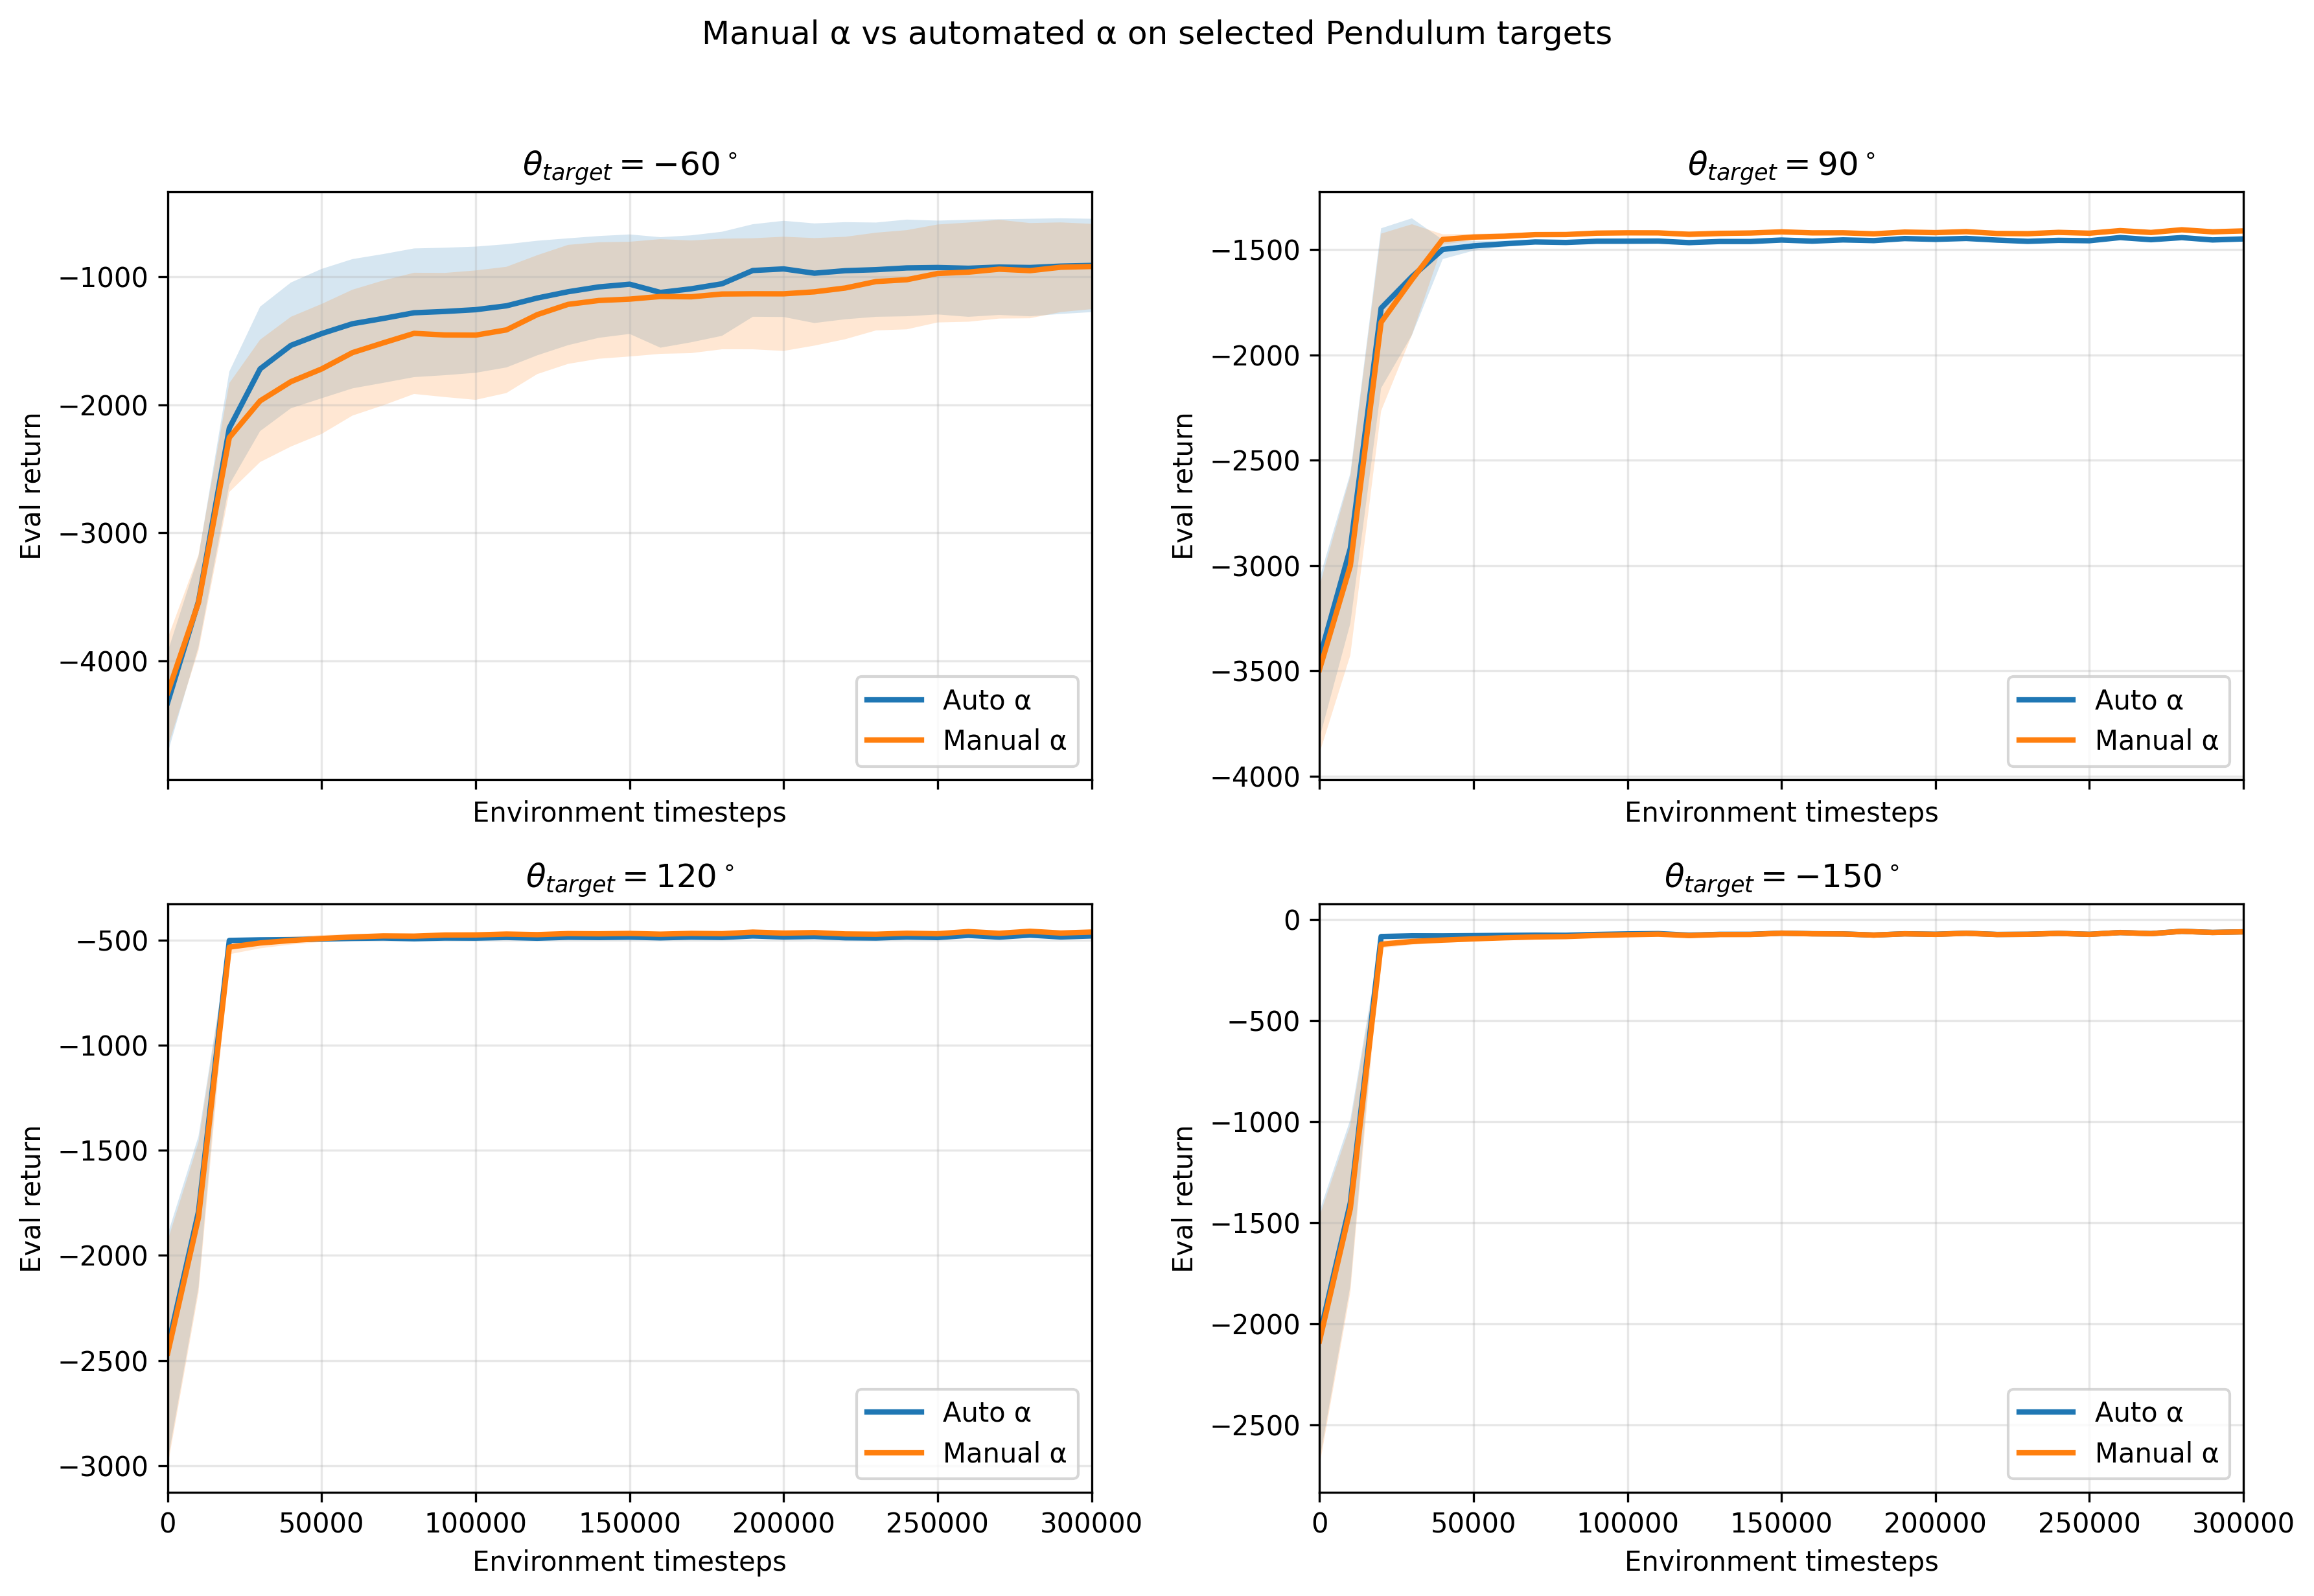
\includegraphics[width=0.88\textwidth]{P3_manual_vs_auto_eval_return_panels.png}
\caption{Manual $\alpha$ vs.\ auto-tuning (mean $\pm$ 95\% CI).}
\label{fig:pendulum_manual_auto}
\end{figure}

Manual $\alpha$ gives modest gains for $90^\circ$ ($-1429$ vs $-1469$) and $120^\circ$ ($-478$ vs $-497$). For $-150^\circ$, both methods are essentially equivalent. For $-60^\circ$, both show wide confidence intervals, making the comparison inconclusive. Auto-tuning is a strong default: it avoids the 72-run search cost and remains competitive across all targets. Manual tuning can help specific targets when one is willing to invest in the additional pilot experiments.

\subsection{Reward Scaling}

For $\theta=90^\circ$ with scales $0.1\times$ and $10\times$:

\begin{figure}[H]
\centering
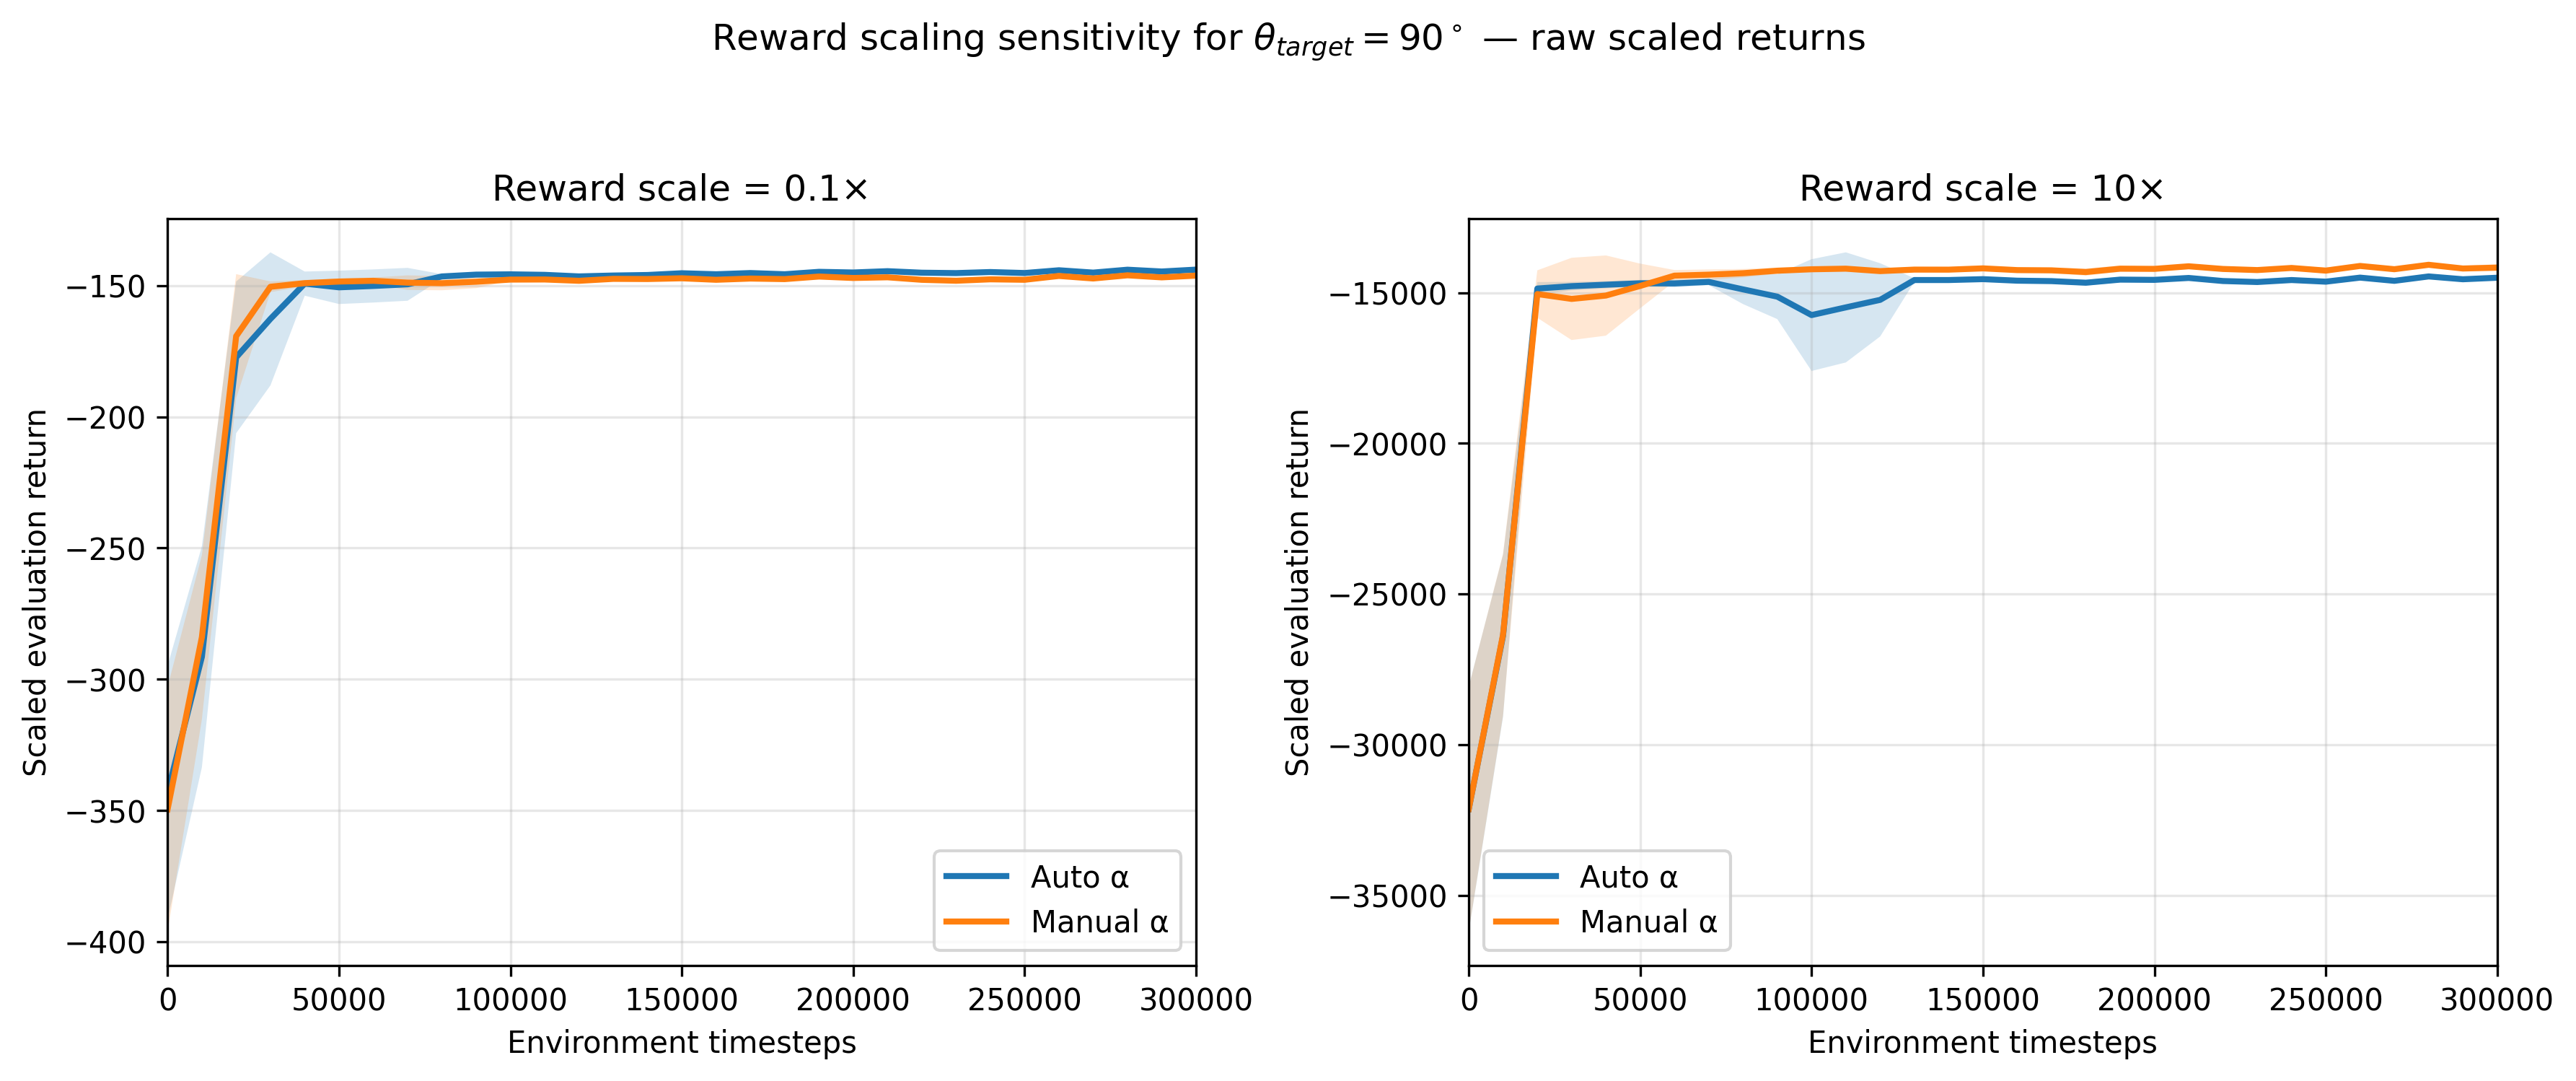
\includegraphics[width=0.88\textwidth]{P5_reward_scaling_eval_return_panels_FIXED.png}
\caption{Reward scaling: auto vs.\ manual $\alpha$ at $0.1\times$ and $10\times$.}
\label{fig:pendulum_reward_scaling}
\end{figure}

\textbf{Does manual $\alpha$ adapt?} No. Manual $\alpha$ was tuned at reward scale $1\times$. Scaling the reward by $10\times$ makes the entropy term $\alpha\mathcal{H}$ relatively ten times weaker, reducing exploration. Scaling by $0.1\times$ makes it ten times stronger, potentially over-exploring. In both cases the effective reward-entropy balance shifts away from the tuned optimum.

\textbf{Does auto $\alpha$ adapt?} Mostly yes. Automatic tuning adjusts the entropy temperature to maintain target entropy regardless of reward scale. However, reward scaling also changes critic target magnitudes and gradient scales, which affect learning dynamics independently of entropy. At $0.1\times$: auto-$\alpha$ achieves $-145.3$, manual achieves $-147.7$. At $10\times$: manual achieves $-14359.8$, auto achieves $-14674.9$---the auto curve shows a temporary mid-training dip from large critic gradients. Automatic tuning improves robustness but does not fully remove sensitivity to reward magnitude.

% ============================================================
% SECTION 2.2: LUNAR LANDER
% ============================================================
\section{Section 2.2: Lunar Lander}

\subsection{Experimental Setup}

We used \texttt{LunarLander-v3} in both continuous and discrete action settings. For the continuous-action experiments, SAC uses a tanh-squashed Gaussian actor, twin Q-critics, clipped double-Q targets, target networks, reparameterized actor updates, Adam optimizer, and automatic entropy-temperature tuning. The main hyperparameters were hidden layers $(256,256)$, learning rates $3\times 10^{-4}$, discount factor $\gamma=0.99$, target update coefficient $\tau=0.005$, batch size 256, replay buffer size $10^6$, and 10K initial random exploration steps. Evaluation was done every 10K environment steps using 20 deterministic offline episodes.

\begin{table}[h]
\centering
\caption{Summary of LunarLander experiments. Values are final evaluation returns.}
\small
\begin{tabular}{lcccc}
\toprule
Experiment & Action space & Steps & Final return & Main conclusion \\
\midrule
Continuous SAC, auto-$\alpha$ & Continuous & 300K & $176.6 \pm 88.1$ & Learns, but seed-sensitive \\
Hover SAC, fixed $\alpha=0.01$ & Continuous & 600K & $167.3 \pm 84.5$ & Weak recovery after switch \\
Hover SAC, auto-$\alpha$ & Continuous & 600K & $271.1 \pm 5.4$ & Strongest and most stable \\
Discrete SAC & Discrete & 250K & $-758.2 \pm 0.0$ & Unstable / failed run \\
DQN & Discrete & 250K & $128.2 \pm 86.8$ & Learns steadily \\
\bottomrule
\end{tabular}
\end{table}

\subsection{Continuous SAC with Automated Temperature Tuning}

\begin{figure}[H]
    \centering
    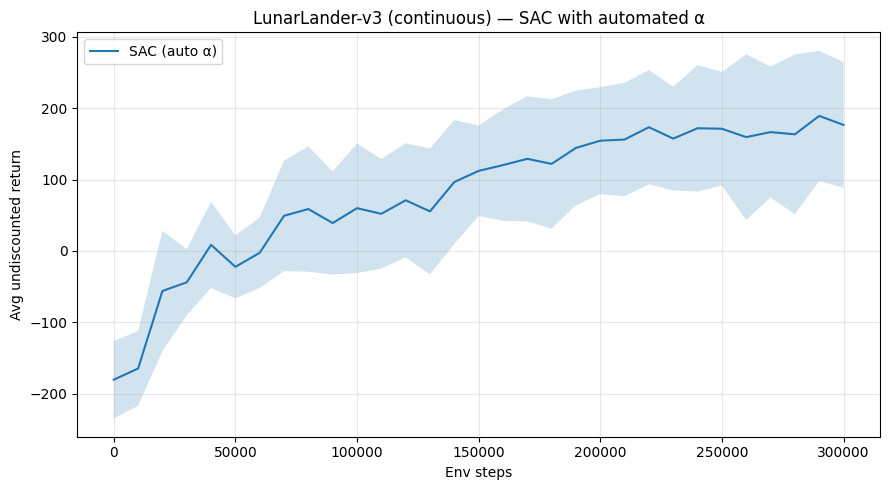
\includegraphics[width=0.72\linewidth]{continuous_sac_auto_alpha.png}
    \caption{Continuous SAC on LunarLander-v3 with automated temperature tuning.}
    \label{fig:lunar-cont-sac}
\end{figure}

Figure~\ref{fig:lunar-cont-sac} shows that continuous SAC learns meaningful control behavior. The average return improves from strongly negative values to approximately $176.6$ by 300K steps. The behavior can be divided into three stages. In the initial stage, the policy fires engines randomly, rotates excessively, and crashes. In the intermediate stage, the agent learns to stabilize and slow its descent---a common local optimum where avoiding crashes gives better return than landing poorly. In the final stage, successful seeds learn controlled descent and attempt to land between the flags. The wide confidence interval shows this final behavior is not equally strong for all seeds.

\subsection{Hover-Box Reward Switch}

We modified the continuous LunarLander environment by adding a one-time hover reward. Initially $+200$ for entering the box $|x|<0.1$, $0.4<|y|<0.6$, then changed to $-100$. We compared fixed $\alpha=0.01$ and automated $\alpha$.

\begin{figure}[H]
    \centering
    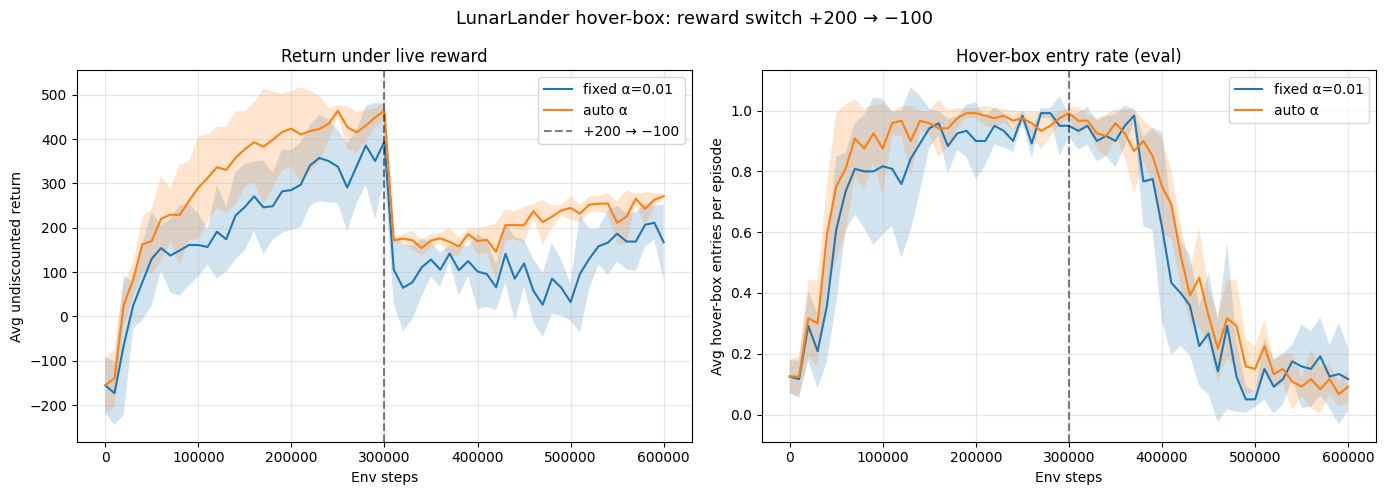
\includegraphics[width=\linewidth]{hover_return_hits.png}
    \caption{Hover-box reward-switch experiment. Left: evaluation return. Right: hover-box entry rate. Dashed line marks the switch from $+200$ to $-100$.}
    \label{fig:hover-return-hits}
\end{figure}

Before the switch, both agents exploit the hover box. After the switch, auto-$\alpha$ recovers to $271.1 \pm 5.4$, while fixed-$\alpha$ remains noisy at $167.3 \pm 84.5$. This is the strongest result in this section.

\begin{figure}[H]
    \centering
    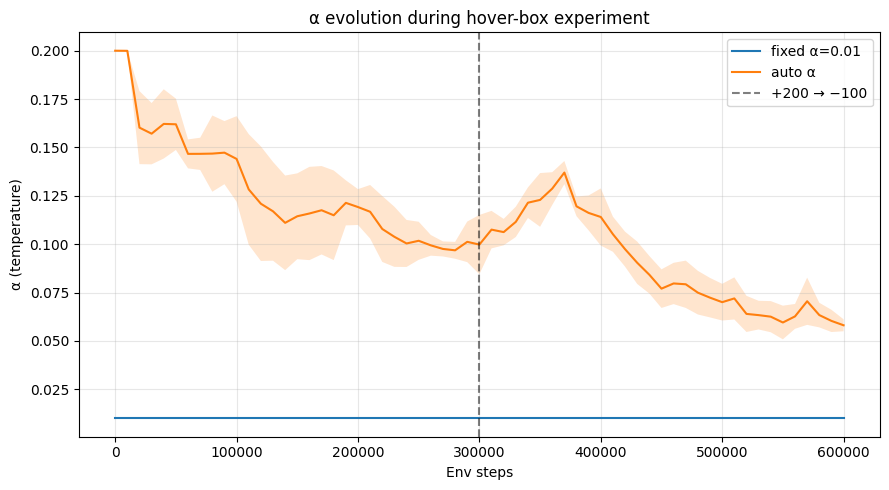
\includegraphics[width=0.72\linewidth]{hover_alpha_evolution.png}
    \caption{Evolution of $\alpha$ during the hover-box experiment. Auto-$\alpha$ adapts around the reward switch.}
    \label{fig:hover-alpha}
\end{figure}

Figure~\ref{fig:hover-alpha} explains why: auto-$\alpha$ increases entropy around the switch, enabling exploration away from the old local optimum. This supports the maximum-entropy interpretation of SAC:
\[
J(\pi)=\mathbb{E}_{\pi}\left[\sum_t r_t + \alpha \mathcal{H}(\pi(\cdot|s_t))\right].
\]
Entropy regularization discourages premature determinism and improves robustness when the reward landscape changes.

\subsection{Discrete SAC Formulation}

For the discrete-action version, the Gaussian policy is replaced by a categorical policy $\pi(a|s)$. Since the action set is small, expectations are computed exactly:
\[
y = r + \gamma(1-d)\sum_{a'} \pi(a'|s')\left[\min_i Q_i^{\mathrm{targ}}(s',a') - \alpha \log \pi(a'|s')\right].
\]
\[
J_\pi = \mathbb{E}_{s}\left[\sum_a \pi(a|s)\left(\alpha \log \pi(a|s) - \min_i Q_i(s,a)\right)\right].
\]

\subsection{Discrete SAC vs.\ DQN}

\begin{figure}[H]
    \centering
    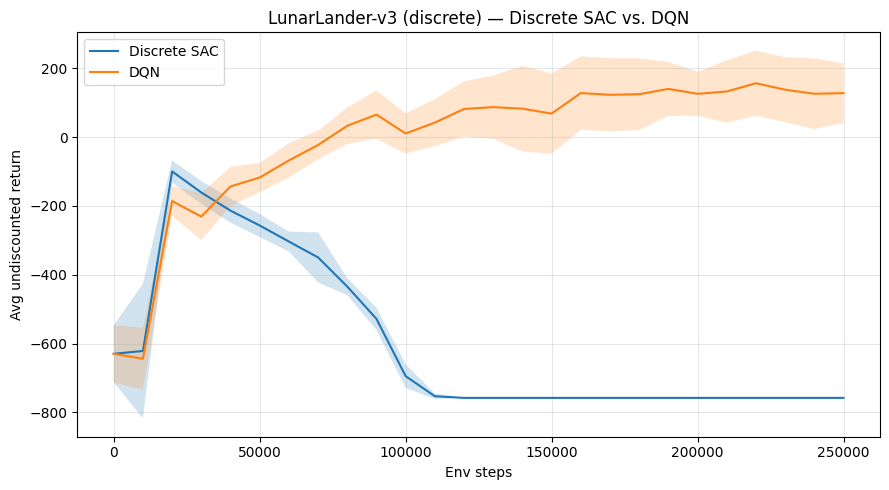
\includegraphics[width=0.78\linewidth]{discrete_sac_vs_dqn.png}
    \caption{Discrete SAC vs.\ DQN on discrete-action LunarLander-v3.}
    \label{fig:disc-sac-dqn}
\end{figure}

DQN learns steadily and reaches approximately $128.2 \pm 86.8$. Our Discrete SAC run collapses to $-758.2$ after around 100K steps due to alpha explosion. We investigated the root cause: with \texttt{target\_entropy\_ratio}$=0.50$, the target entropy is $0.50\times\ln(4)=0.693$, but actual policy entropy stabilizes near $1.35$ (close to maximum entropy $\ln(4)=1.386$). Since entropy consistently exceeds the target, the alpha update pushes $\alpha$ upward in a positive feedback loop ($\alpha: 0.2 \to 8.5$M), causing critic loss to diverge.

We attempted a fix by setting \texttt{target\_entropy\_ratio}$=0.98$ (target entropy $=1.36$, matching the observed entropy). The agent initially showed improvement (return rose from $-580$ to $-17$ at 10K steps), but subsequently collapsed to the same $-758.2$ level. This suggests the instability is not purely due to the entropy target mismatch---the critic loss scaling and actor-critic coupling under large Q-values also contribute to the divergence. A more robust fix would likely require gradient clipping, alpha clamping, or a different critic architecture.

\textbf{Preference for discrete actions.} Based on our results, DQN is clearly preferred for discrete LunarLander:
\begin{itemize}
    \item \textbf{Performance:} DQN achieves $+128$ mean return vs.\ Discrete SAC's $-758$.
    \item \textbf{Sample efficiency:} DQN improves steadily throughout training; Discrete SAC collapses after initial progress.
    \item \textbf{Ease of implementation:} DQN requires only a Q-network, target network, and $\epsilon$-greedy exploration. Discrete SAC adds a categorical actor, twin critics, entropy temperature, and entropy-target tuning---all of which increase sensitivity to hyperparameters.
\end{itemize}
Discrete SAC remains theoretically attractive for its principled exploration via entropy maximization, but in practice it requires careful tuning of the entropy target and alpha dynamics that DQN avoids entirely.

% ============================================================
% SECTION 2.3: REACHER
% ============================================================
\section{Section 2.3: Reacher}

\subsection{Setup}

We used \texttt{reacher-easy} from the DeepMind Control Suite. The task consists of a two-joint robotic arm, and the desired behavior is to reach the target sphere quickly and remain there. We trained three SAC agents corresponding to three reward formulations:
\begin{align}
R_a(s,a) &= \begin{cases}1, & \text{fingertip in target},\\ -\lVert x_{\text{goal}} - x_{\text{finger}}\rVert - \lVert a\rVert^2, & \text{otherwise},\end{cases} \\
R_b(s,a) &= \begin{cases}1, & \text{fingertip in target},\\ 0, & \text{otherwise},\end{cases} \\
R_c(s,a) &= -1 \quad \text{per step until the target is reached with low velocity.}
\end{align}

For $R_a$ and $R_b$, episodes are fixed-length with horizon 1000. For $R_c$, if the agent does not reach the target within 1000 steps, we reset the arm while keeping the same target and apply a timeout penalty of $-20$. All agents trained for 500K steps using the same SAC setup. For cross-evaluation, each trained policy was evaluated under all three reward formulations.

\subsection{Self-Evaluation}

\begin{figure}[H]
    \centering
    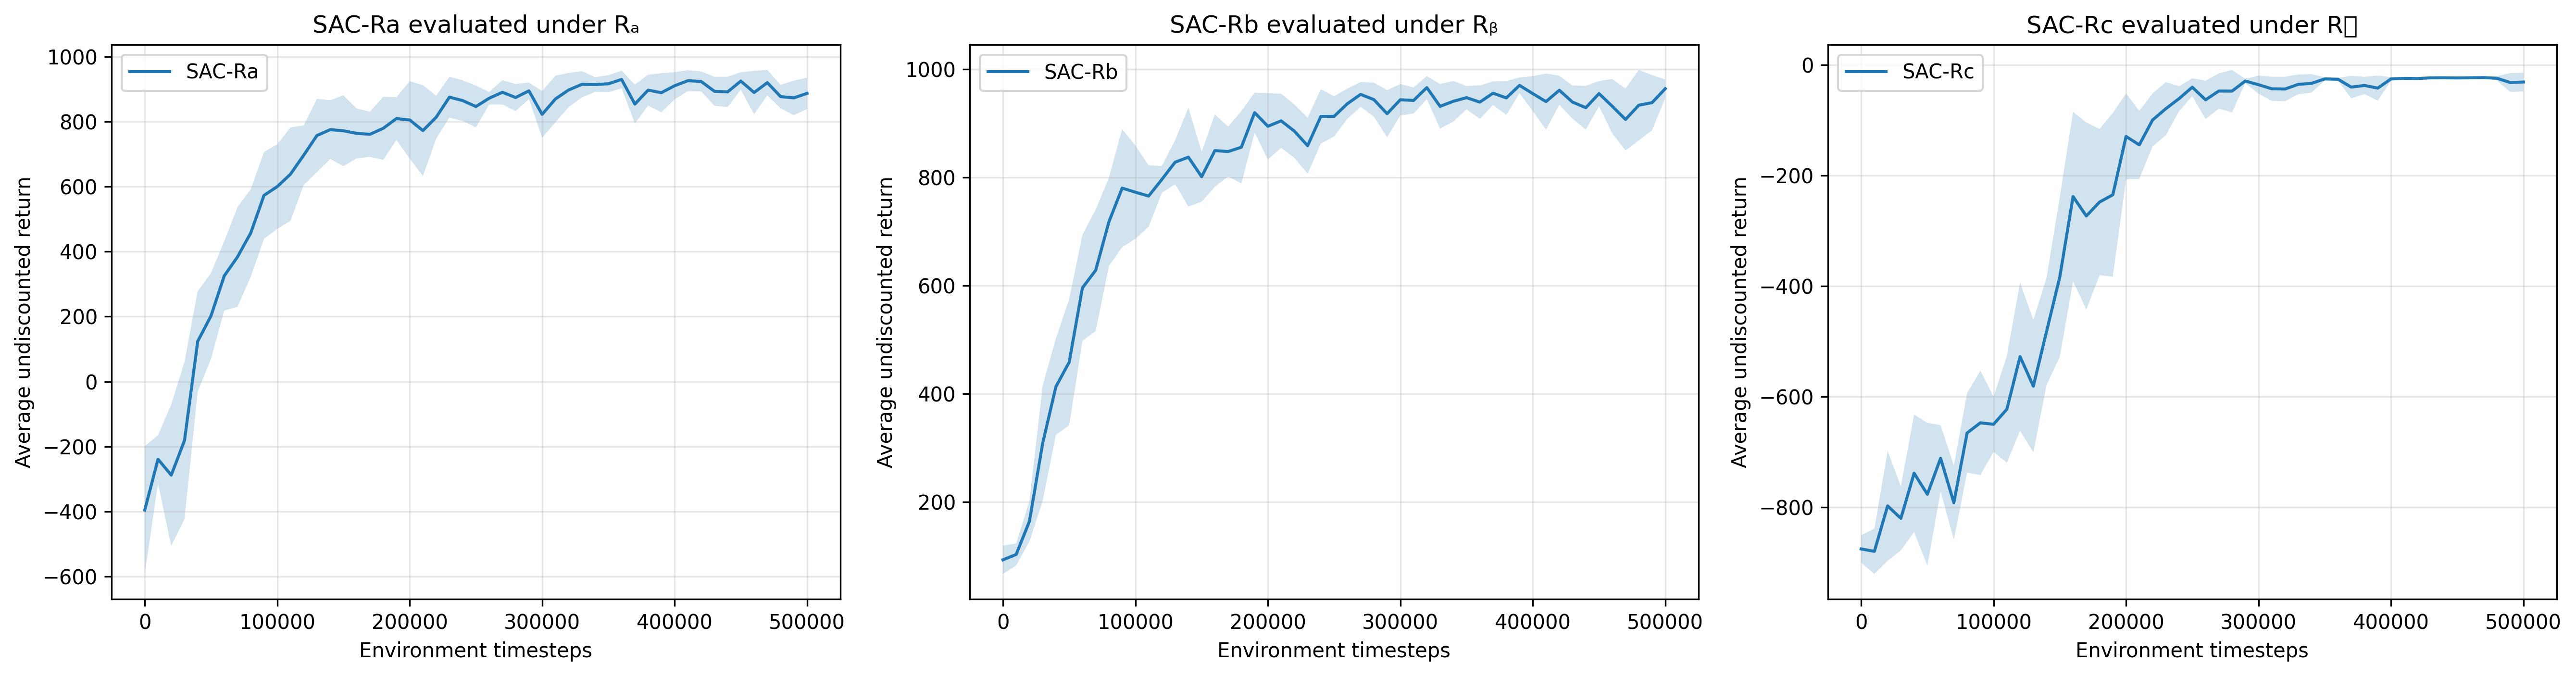
\includegraphics[width=\textwidth]{reacher_self_eval_combined.png}
    \caption{Self-evaluation: each agent evaluated under the reward it was trained with.}
    \label{fig:reacher-self-eval}
\end{figure}

SAC-$R_b$ learns fastest and reaches the highest self-evaluation return ($\sim$950). SAC-$R_a$ converges steadily to $\sim$900. SAC-$R_c$ starts very negative but improves toward zero (better for $R_c$ since the reward is $-1$ per step until success). Learning is faster for $R_a$ and $R_b$ because they provide informative signal before the target is reached, while $R_c$ gives a harsh constant $-1$ until the agent discovers successful reaching.

\subsection{Final-Policy Behavioral Metrics}

\begin{figure}[H]
    \centering
    \begin{subfigure}{0.48\textwidth}
        \centering
        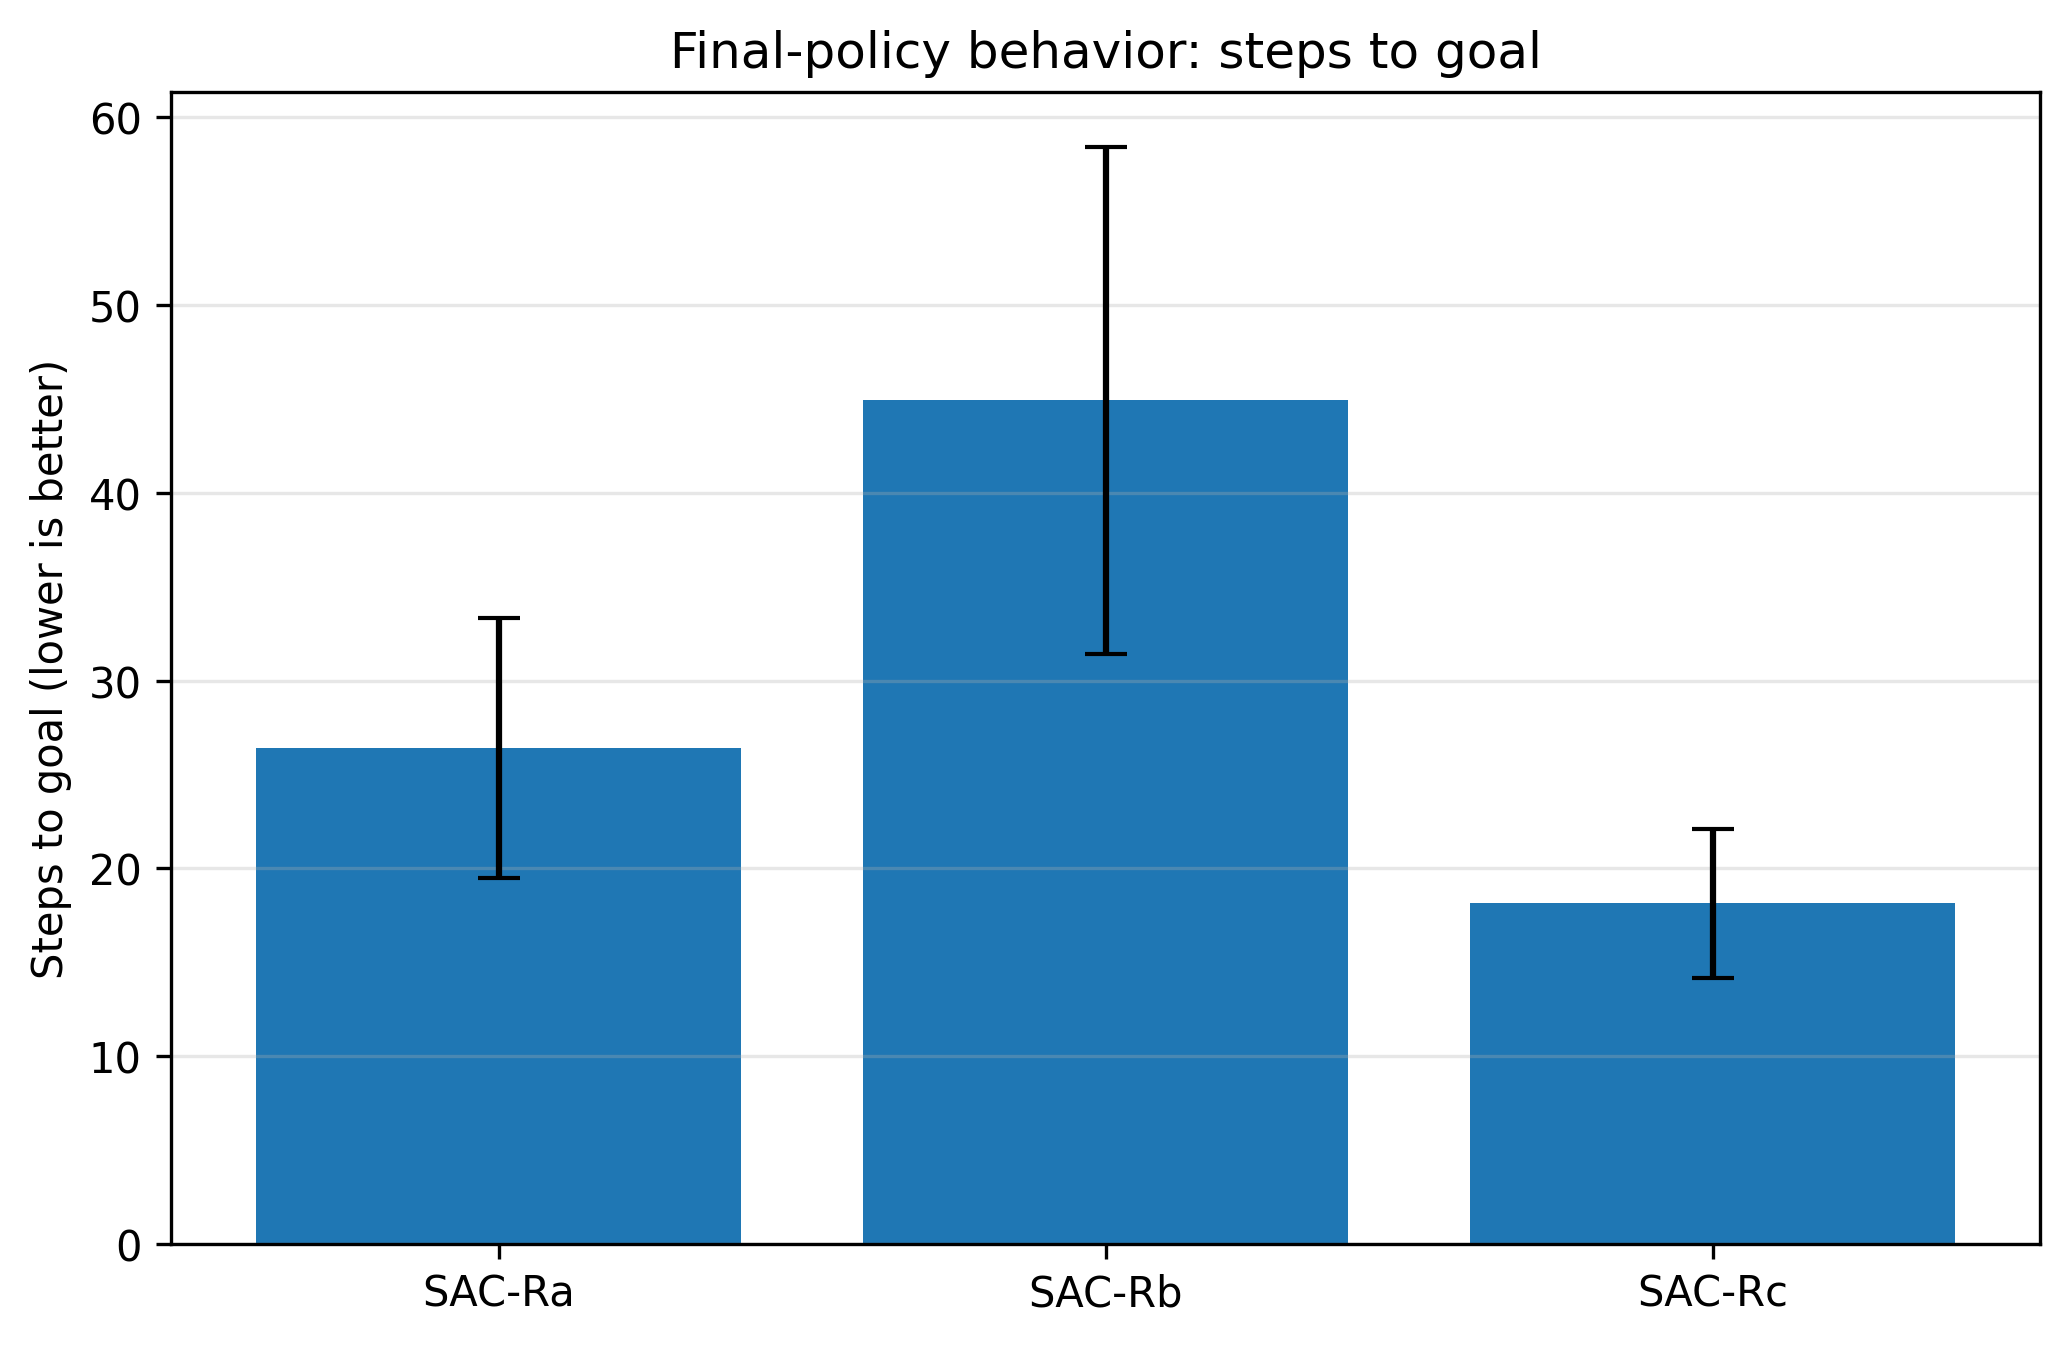
\includegraphics[width=\linewidth]{reacher_behavior_steps_to_goal.png}
        \caption{Steps to goal. Lower is better.}
    \end{subfigure}
    \hfill
    \begin{subfigure}{0.48\textwidth}
        \centering
        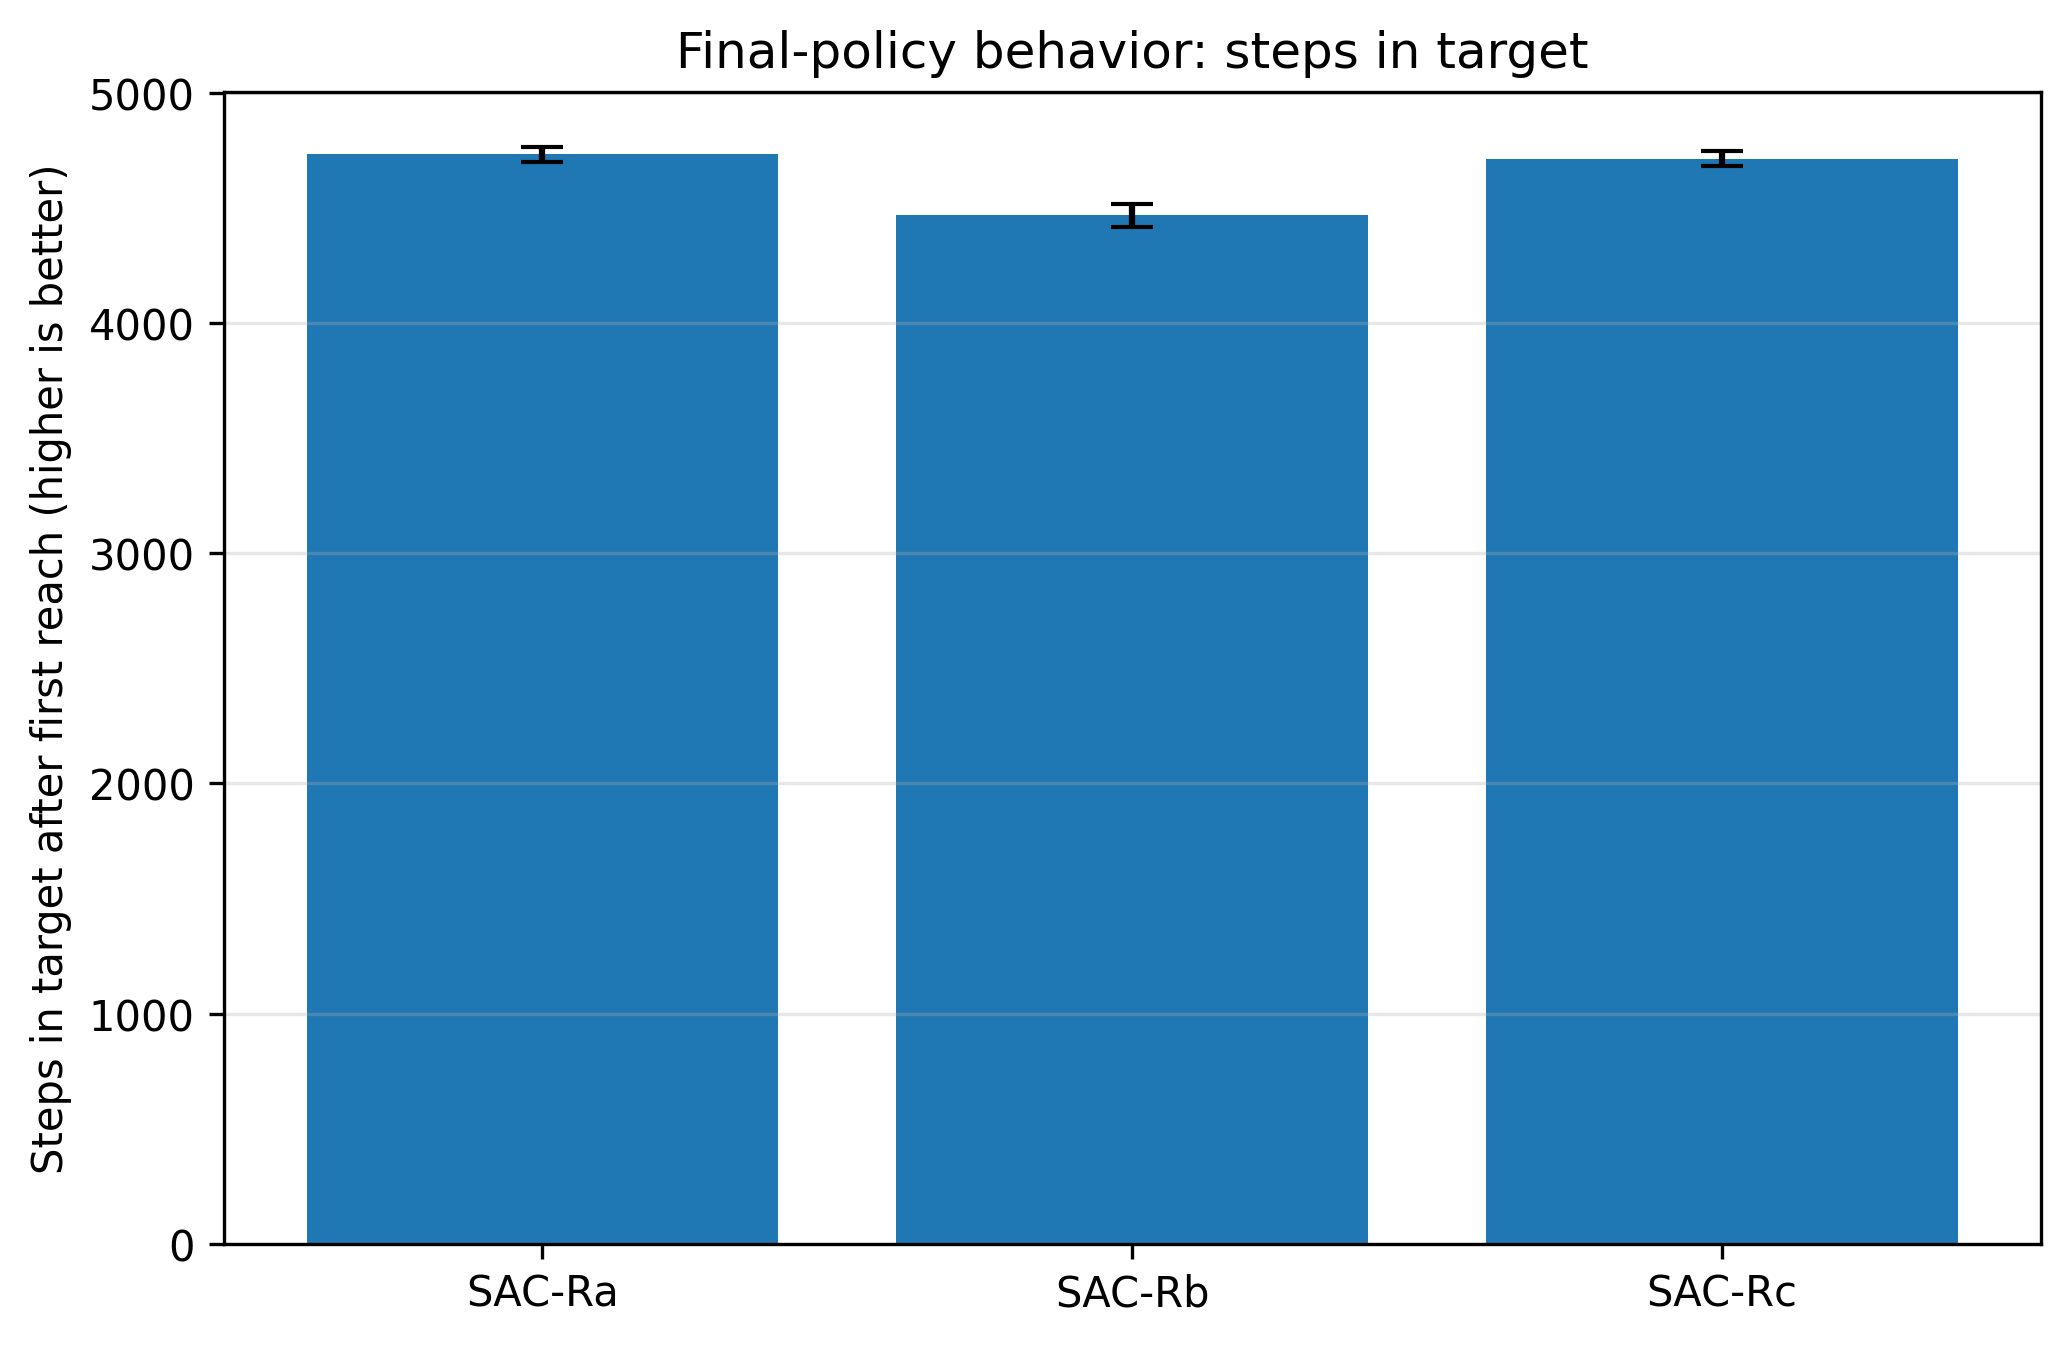
\includegraphics[width=\linewidth]{reacher_behavior_steps_in_target.png}
        \caption{Steps in target after first reach. Higher is better.}
    \end{subfigure}
    \caption{Final-policy diagnostics using 500 evaluation episodes of length 5000.}
    \label{fig:reacher-behavior}
\end{figure}

SAC-$R_c$ reaches the target fastest ($\sim$18 steps), as expected because $R_c$ directly penalizes time. SAC-$R_a$ is second ($\sim$25--30 steps), while SAC-$R_b$ is slower ($\sim$45 steps) with higher variance. For steps-in-target, all three policies remain inside the target for most of the 5000-step horizon. SAC-$R_c$ is best for fast reaching, while SAC-$R_a$ gives the most balanced reach-and-stay behavior.

\subsection{Cross-Evaluation}

\begin{figure}[H]
    \centering
    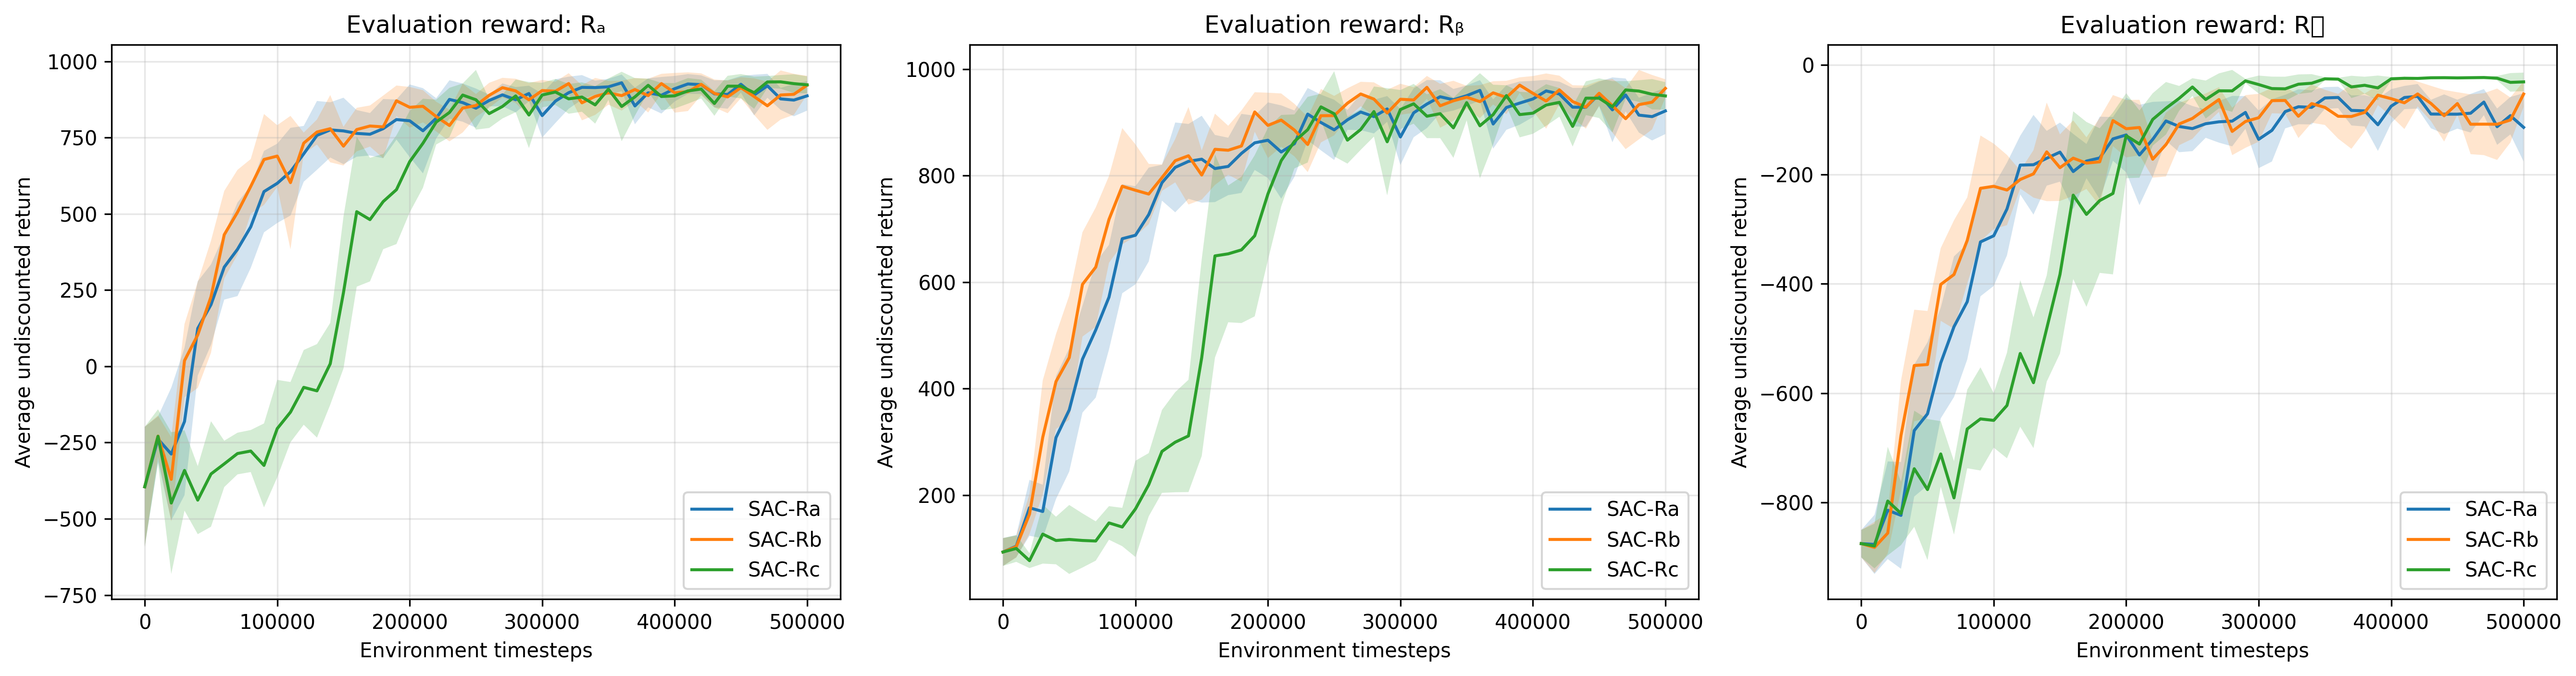
\includegraphics[width=\textwidth]{reacher_cross_eval_combined.png}
    \caption{Cross-evaluation: each subplot fixes the evaluation reward and compares SAC-$R_a$, SAC-$R_b$, and SAC-$R_c$.}
    \label{fig:reacher-cross-eval}
\end{figure}

Under $R_a$ and $R_b$ evaluation, all three policies converge to similar final returns---the rewards are partially aligned since all encode target-reaching behavior. Under $R_c$ evaluation, SAC-$R_c$ achieves the best final performance because it directly optimizes time-to-goal. SAC-$R_a$ and SAC-$R_b$ improve substantially but remain slightly worse under the time-to-goal metric.

\paragraph{Overall comparison.}
In terms of ease of specification, $R_b$ is simplest (binary target detection). In terms of learning efficiency, $R_a$ and $R_b$ learn faster early on. In terms of achieving the desired behavior, $R_c$ is best for reaching quickly, while $R_a$ gives the best balanced behavior (reaching, staying, smooth control). We recommend $R_a$ in practice for stable performance, and $R_c$ when minimizing time-to-goal is the primary objective.

% ============================================================
% SECTION 3: PEBBLE (BONUS)
% ============================================================
\section{Section 3 (Bonus): PEBBLE}

PEBBLE learns a reward model from pairwise preferences via the Bradley-Terry model:
\[
P_\psi(\sigma^0 \succ \sigma^1) = \frac{\exp(\sum_t r_\psi(s_t^0,a_t^0))}{\exp(\sum_t r_\psi(s_t^0,a_t^0)) + \exp(\sum_t r_\psi(s_t^1,a_t^1))}.
\]
A reward ensemble of 3 MLPs is trained with cross-entropy loss on teacher labels; SAC then optimizes the learned reward. The teacher is simulated using ground-truth cumulative return. After each reward-model update, all replay buffer rewards are relabelled with the ensemble prediction.

\subsection{PEBBLE on Pendulum}

We compare PEBBLE (budget=200) against SAC with ground-truth reward for $\theta \in \{0,-60,90,120,-150\}^\circ$.

\begin{figure}[H]
\centering
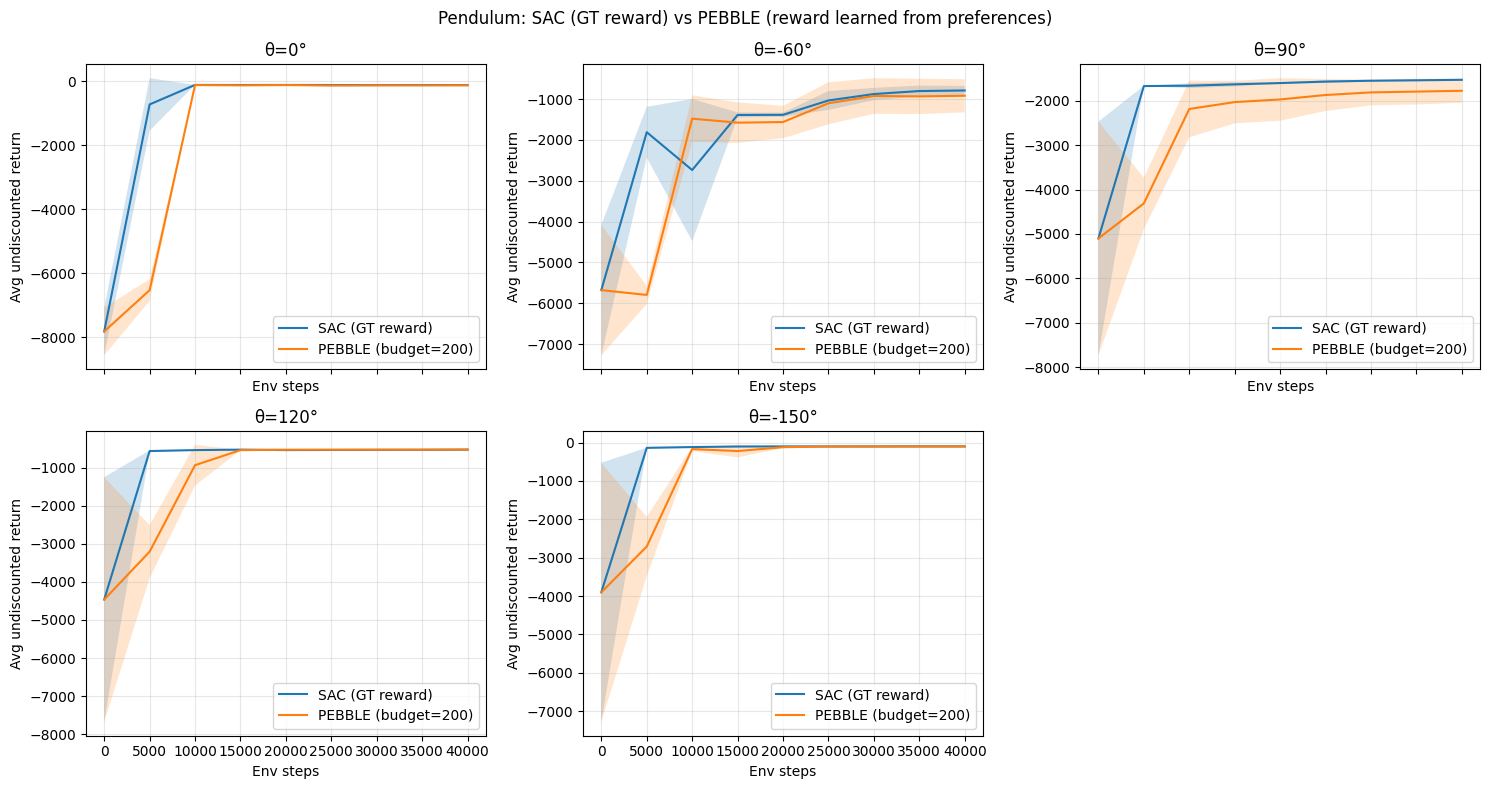
\includegraphics[width=0.92\linewidth]{pebble_pendulum.png}
\caption{PEBBLE vs SAC (GT reward) on Pendulum for five target angles. Y-axis is undiscounted ground-truth return.}
\label{fig:pebble_pend}
\end{figure}

PEBBLE asymptotically matches SAC-GT on all five target angles. For easy targets ($0^\circ$, $-150^\circ$), PEBBLE converges within $\sim$10K steps to the same level as SAC-GT. For harder targets ($-60^\circ$, $90^\circ$, $120^\circ$), both methods converge to similar final returns, though PEBBLE starts slower because (a) the first $\sim$5K steps use intrinsic-only exploration, and (b) the learned reward model is initially less informative than the hand-crafted quadratic. The similar final performance across both methods indicates that 200 preference queries are sufficient for the Pendulum reward structure.

\subsection{Feedback Budget Ablation}

We ablate the feedback budget for $\theta=90^\circ$ with budgets $B \in \{50, 200\}$ and include SAC-GT as reference.

\begin{figure}[H]
\centering
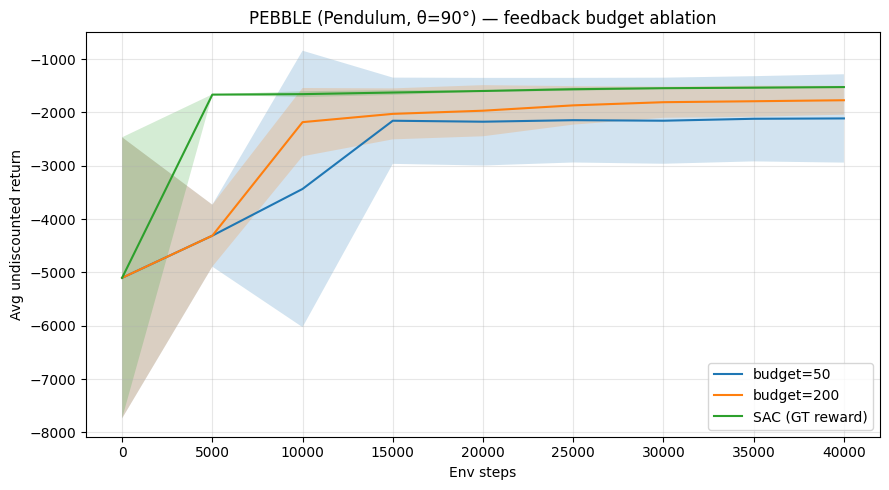
\includegraphics[width=0.78\linewidth]{pebble_budget_ablation.png}
\caption{Budget ablation ($\theta=90^\circ$). SAC-GT converges fastest; $B=200$ nearly matches it; $B=50$ is noisier with wider CI.}
\label{fig:pebble_budget}
\end{figure}

With $B=200$, PEBBLE nearly matches SAC-GT by the end of training, confirming that moderate feedback is sufficient to learn the Pendulum reward structure. With $B=50$, the reward model receives too few labels, resulting in a noisier approximation and wider confidence intervals. The policy still improves but converges to a lower final return. This shows that preference quality and quantity directly affect reward-model accuracy and downstream policy performance, with diminishing returns beyond $\sim$200 queries for this task.

\subsection{PEBBLE on Reacher}

We use three simulated teachers based on $R_a$, $R_b$, and $R_c$ (budget=200).

\begin{figure}[H]
\centering
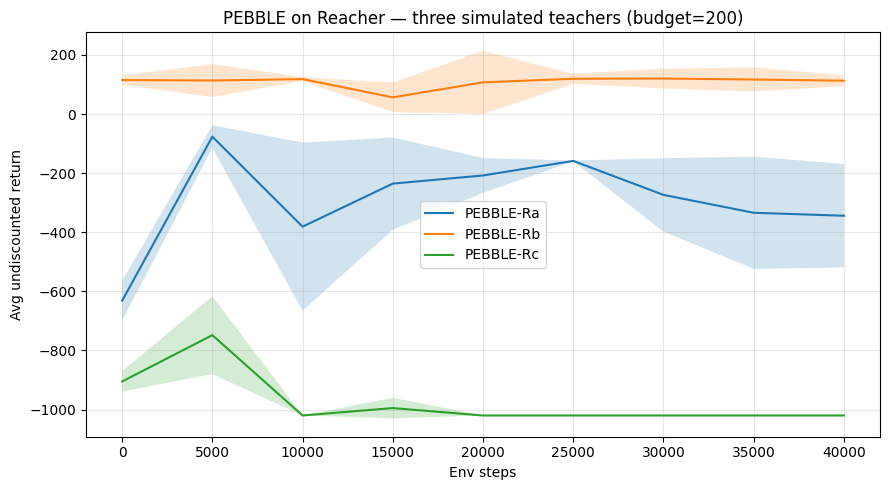
\includegraphics[width=0.78\linewidth]{pebble_reacher.png}
\caption{PEBBLE on Reacher with three simulated teachers. Y-axis is ground-truth return under each teacher's reward.}
\label{fig:pebble_reacher}
\end{figure}

\textbf{PEBBLE-$R_b$} achieves the best and most stable performance ($\sim$120 return), learning quickly and maintaining tight confidence intervals. $R_b$ is a binary indicator (1 if in target, 0 otherwise). Once the agent discovers any successful segment, the preference labels become highly informative: successful segments are clearly preferred over unsuccessful ones. This makes reward learning straightforward.

\textbf{PEBBLE-$R_a$} is unstable and remains negative ($\sim -200$). Although $R_a$ is dense (distance-to-target), the preferences mix distance improvement with action-cost penalties, making the labels more complex. The reward model struggles to disentangle these competing objectives, leading to unstable policy optimization.

\textbf{PEBBLE-$R_c$} collapses to approximately $-1020$ (the timeout return). Since $R_c = -1$ per step until termination, most unsuccessful segments receive nearly identical cumulative returns ($-T$). This makes preference labels weakly informative---the teacher cannot distinguish between two segments that both fail, even if one is closer to succeeding. The reward model therefore learns a near-constant function, and the policy makes no progress.

\textbf{Takeaway:} Simpler, more discriminative reward formulations make better preference teachers. $R_b$'s binary structure produces the clearest preference signal, while $R_c$'s time-penalty structure produces the least informative comparisons.

% ============================================================
% APPENDICES
% ============================================================
\clearpage
\begin{appendix}

\section{Pendulum Behavior Diagnostics}
\label{app:pendulum_diag}

\begin{figure}[H]
\centering
\begin{subfigure}[t]{0.32\textwidth}
    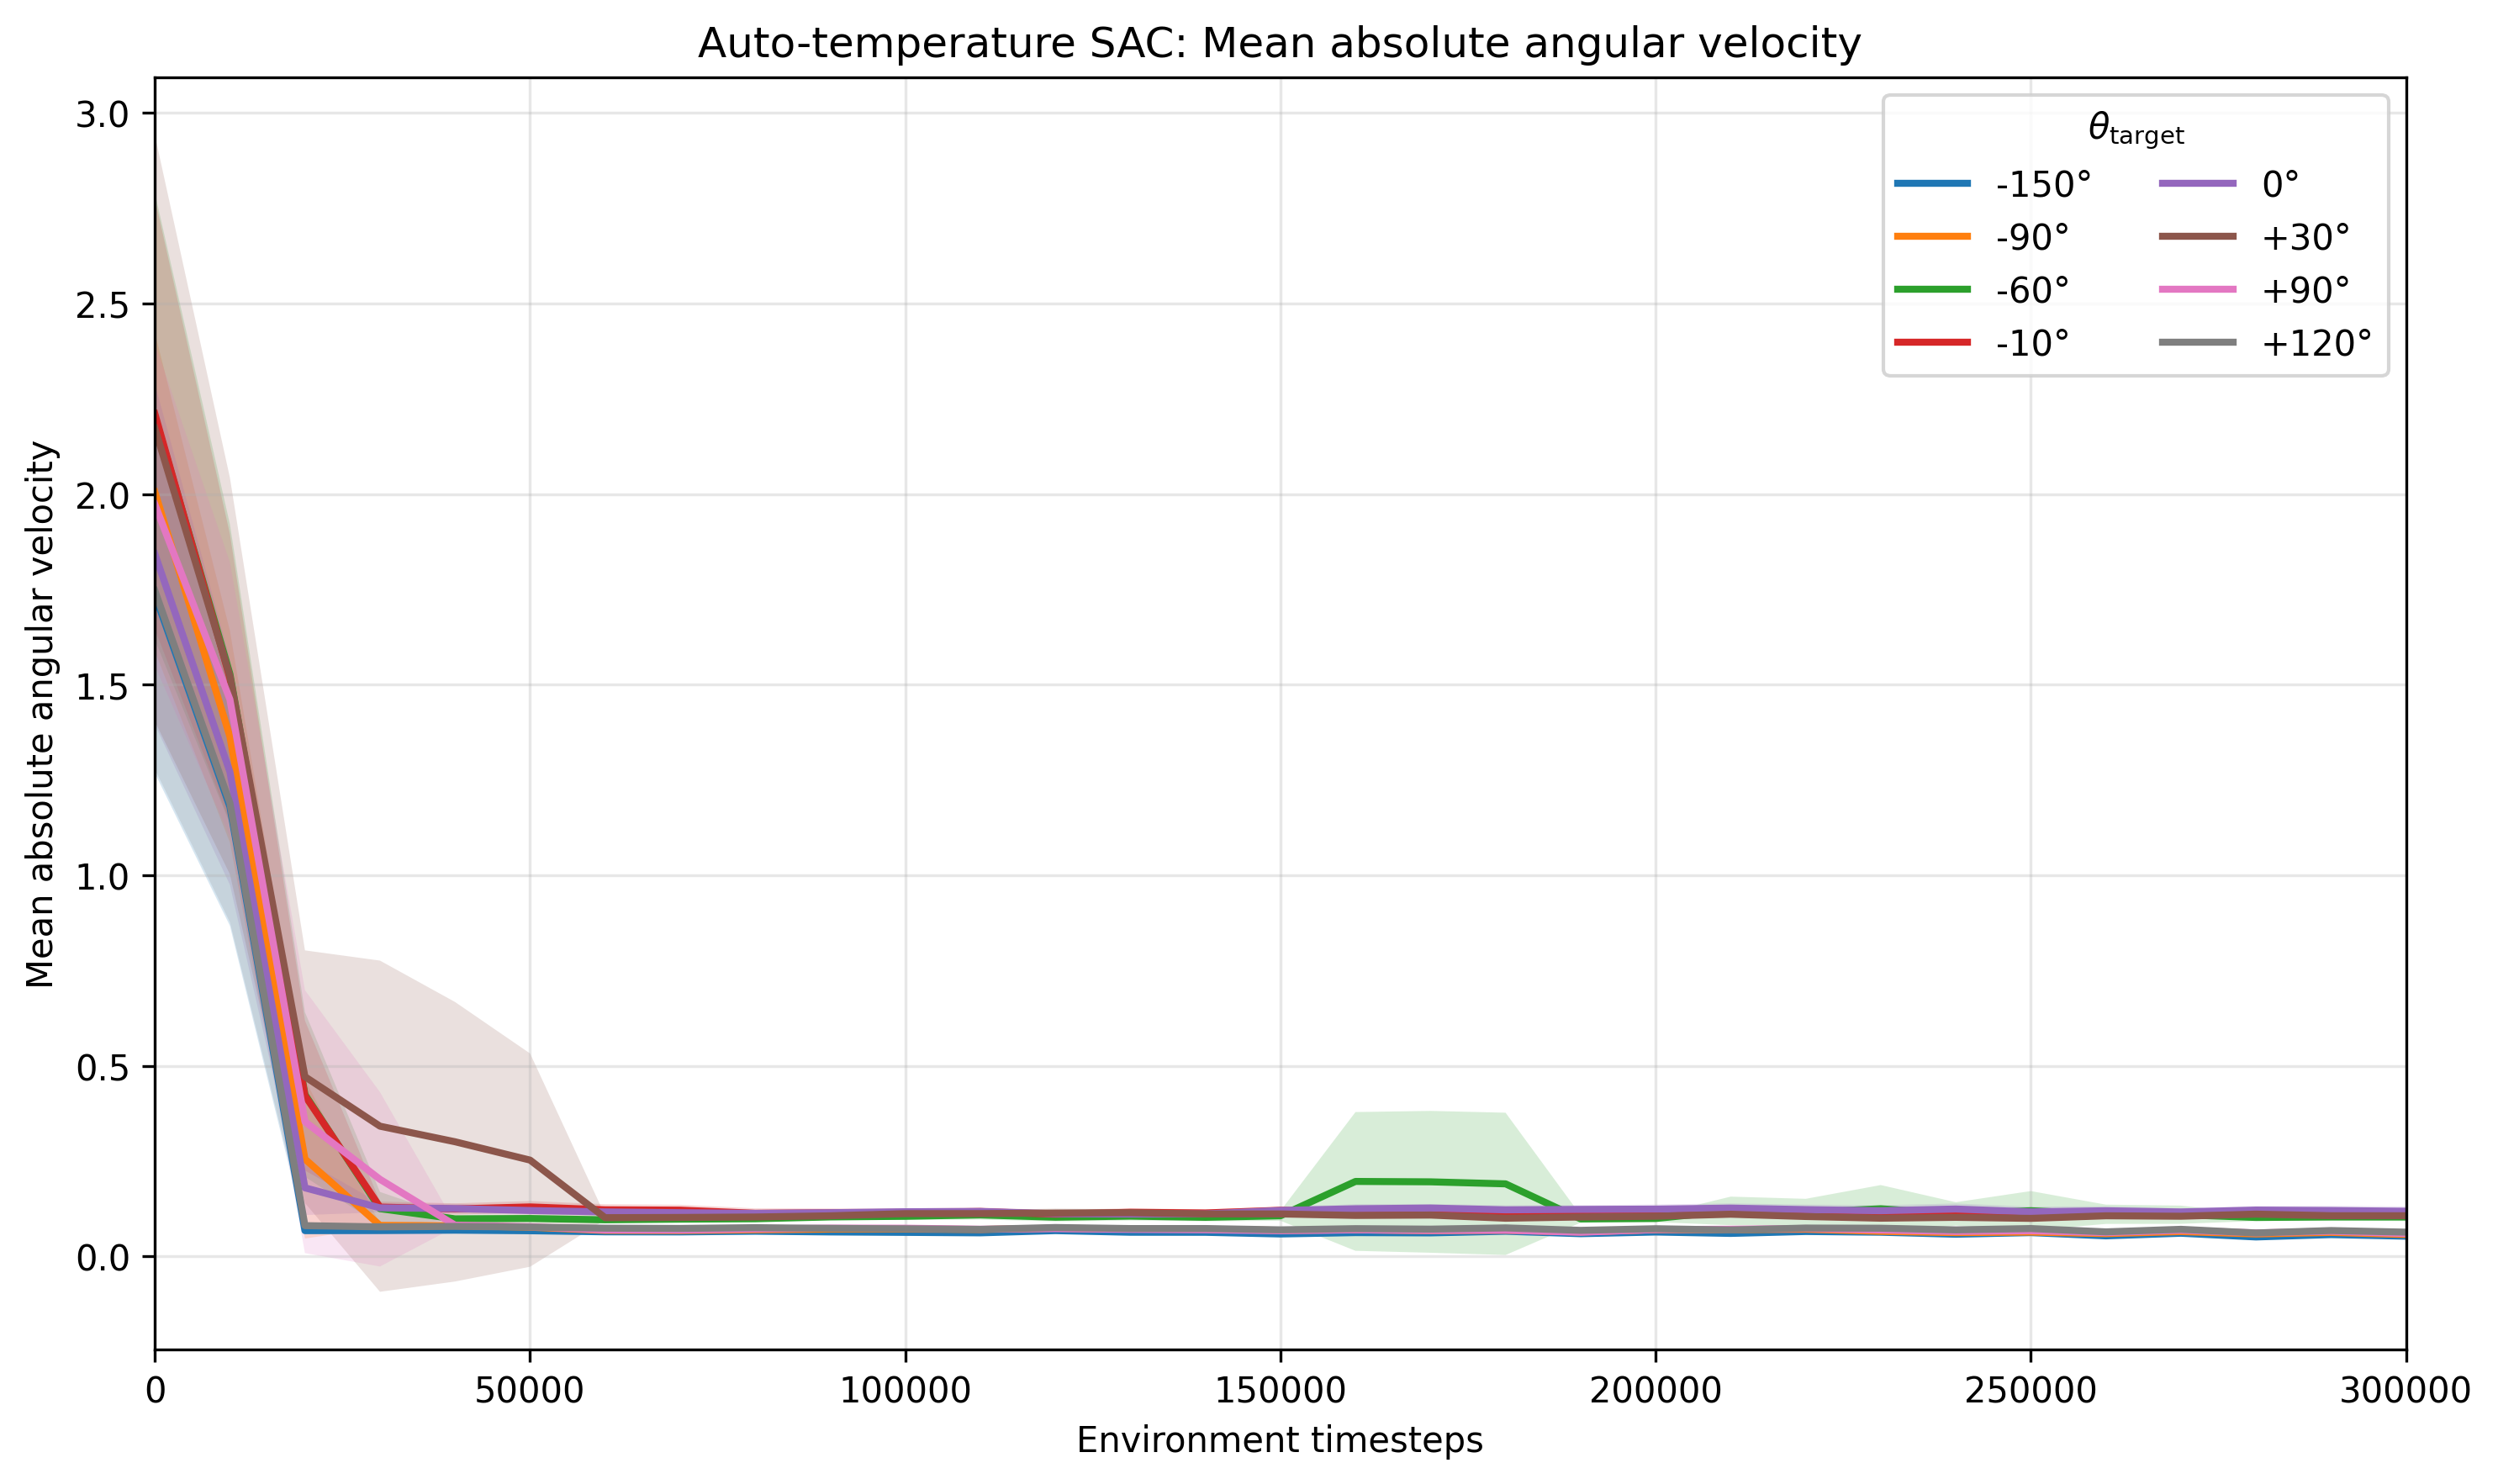
\includegraphics[width=\linewidth]{P1c_auto_all_targets_angular_velocity.png}
    \caption{Angular velocity.}
\end{subfigure}\hfill
\begin{subfigure}[t]{0.32\textwidth}
    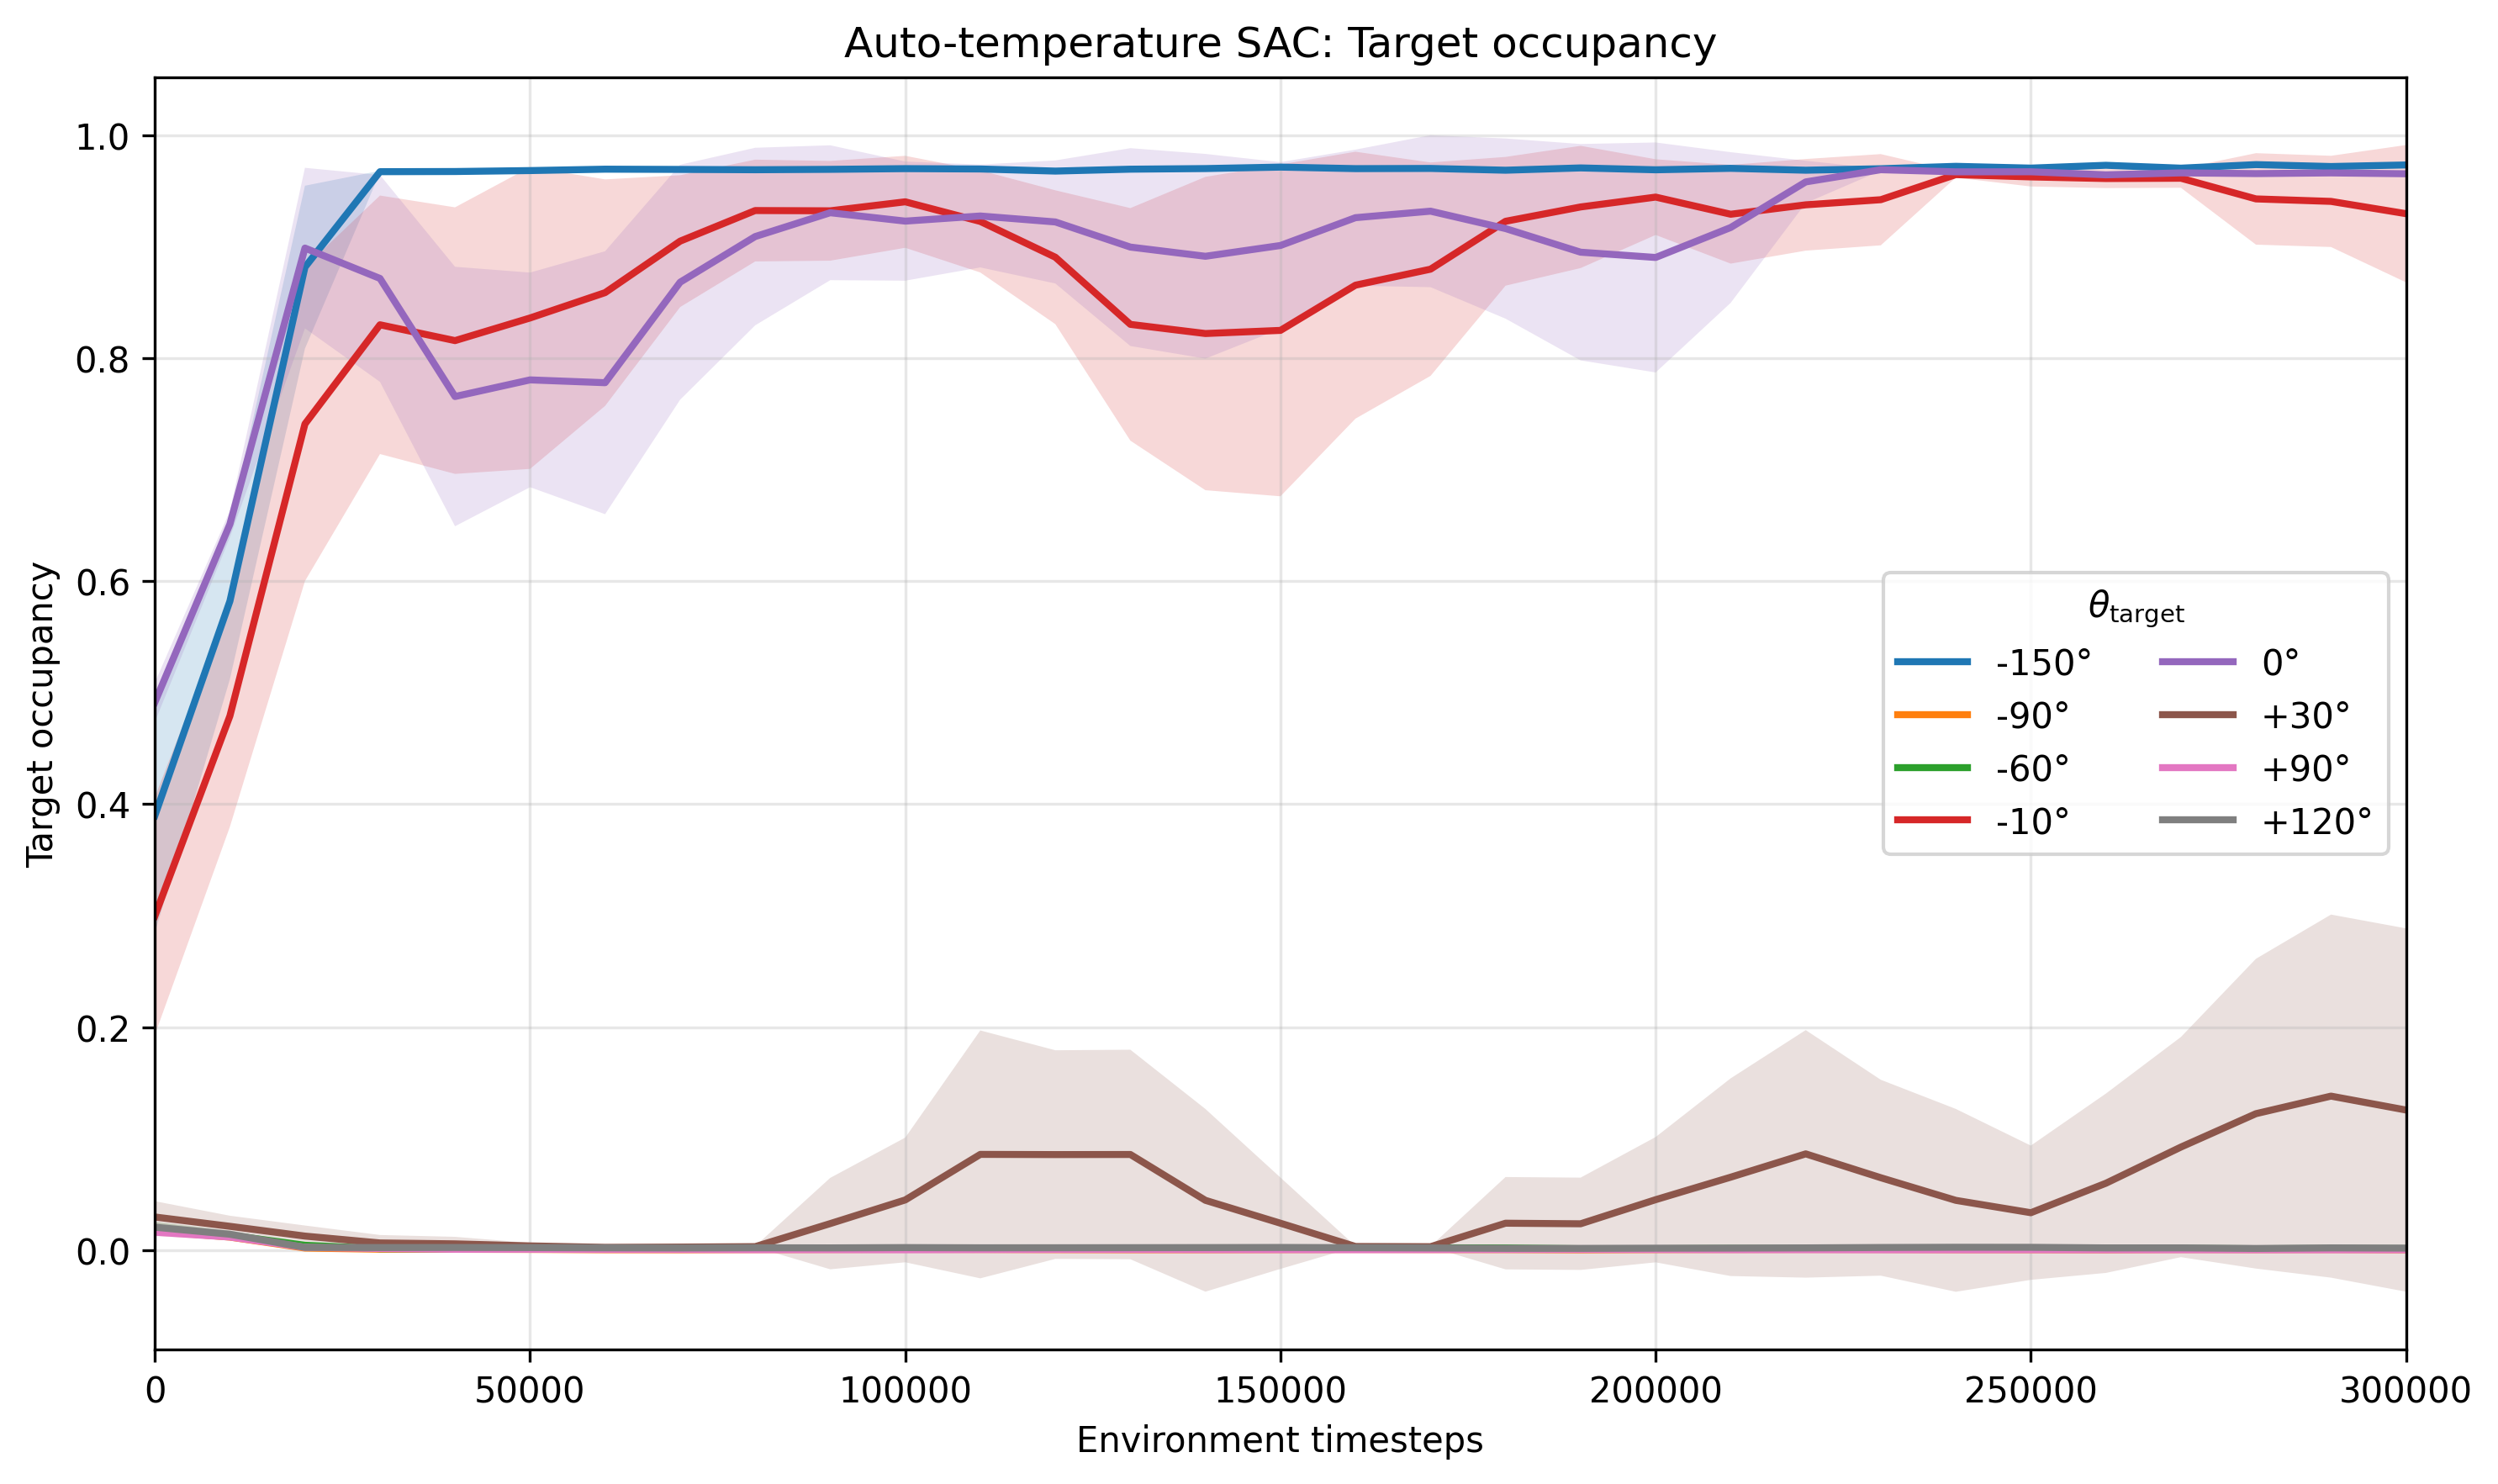
\includegraphics[width=\linewidth]{P1e_auto_all_targets_target_occupancy.png}
    \caption{Target occupancy.}
\end{subfigure}\hfill
\begin{subfigure}[t]{0.32\textwidth}
    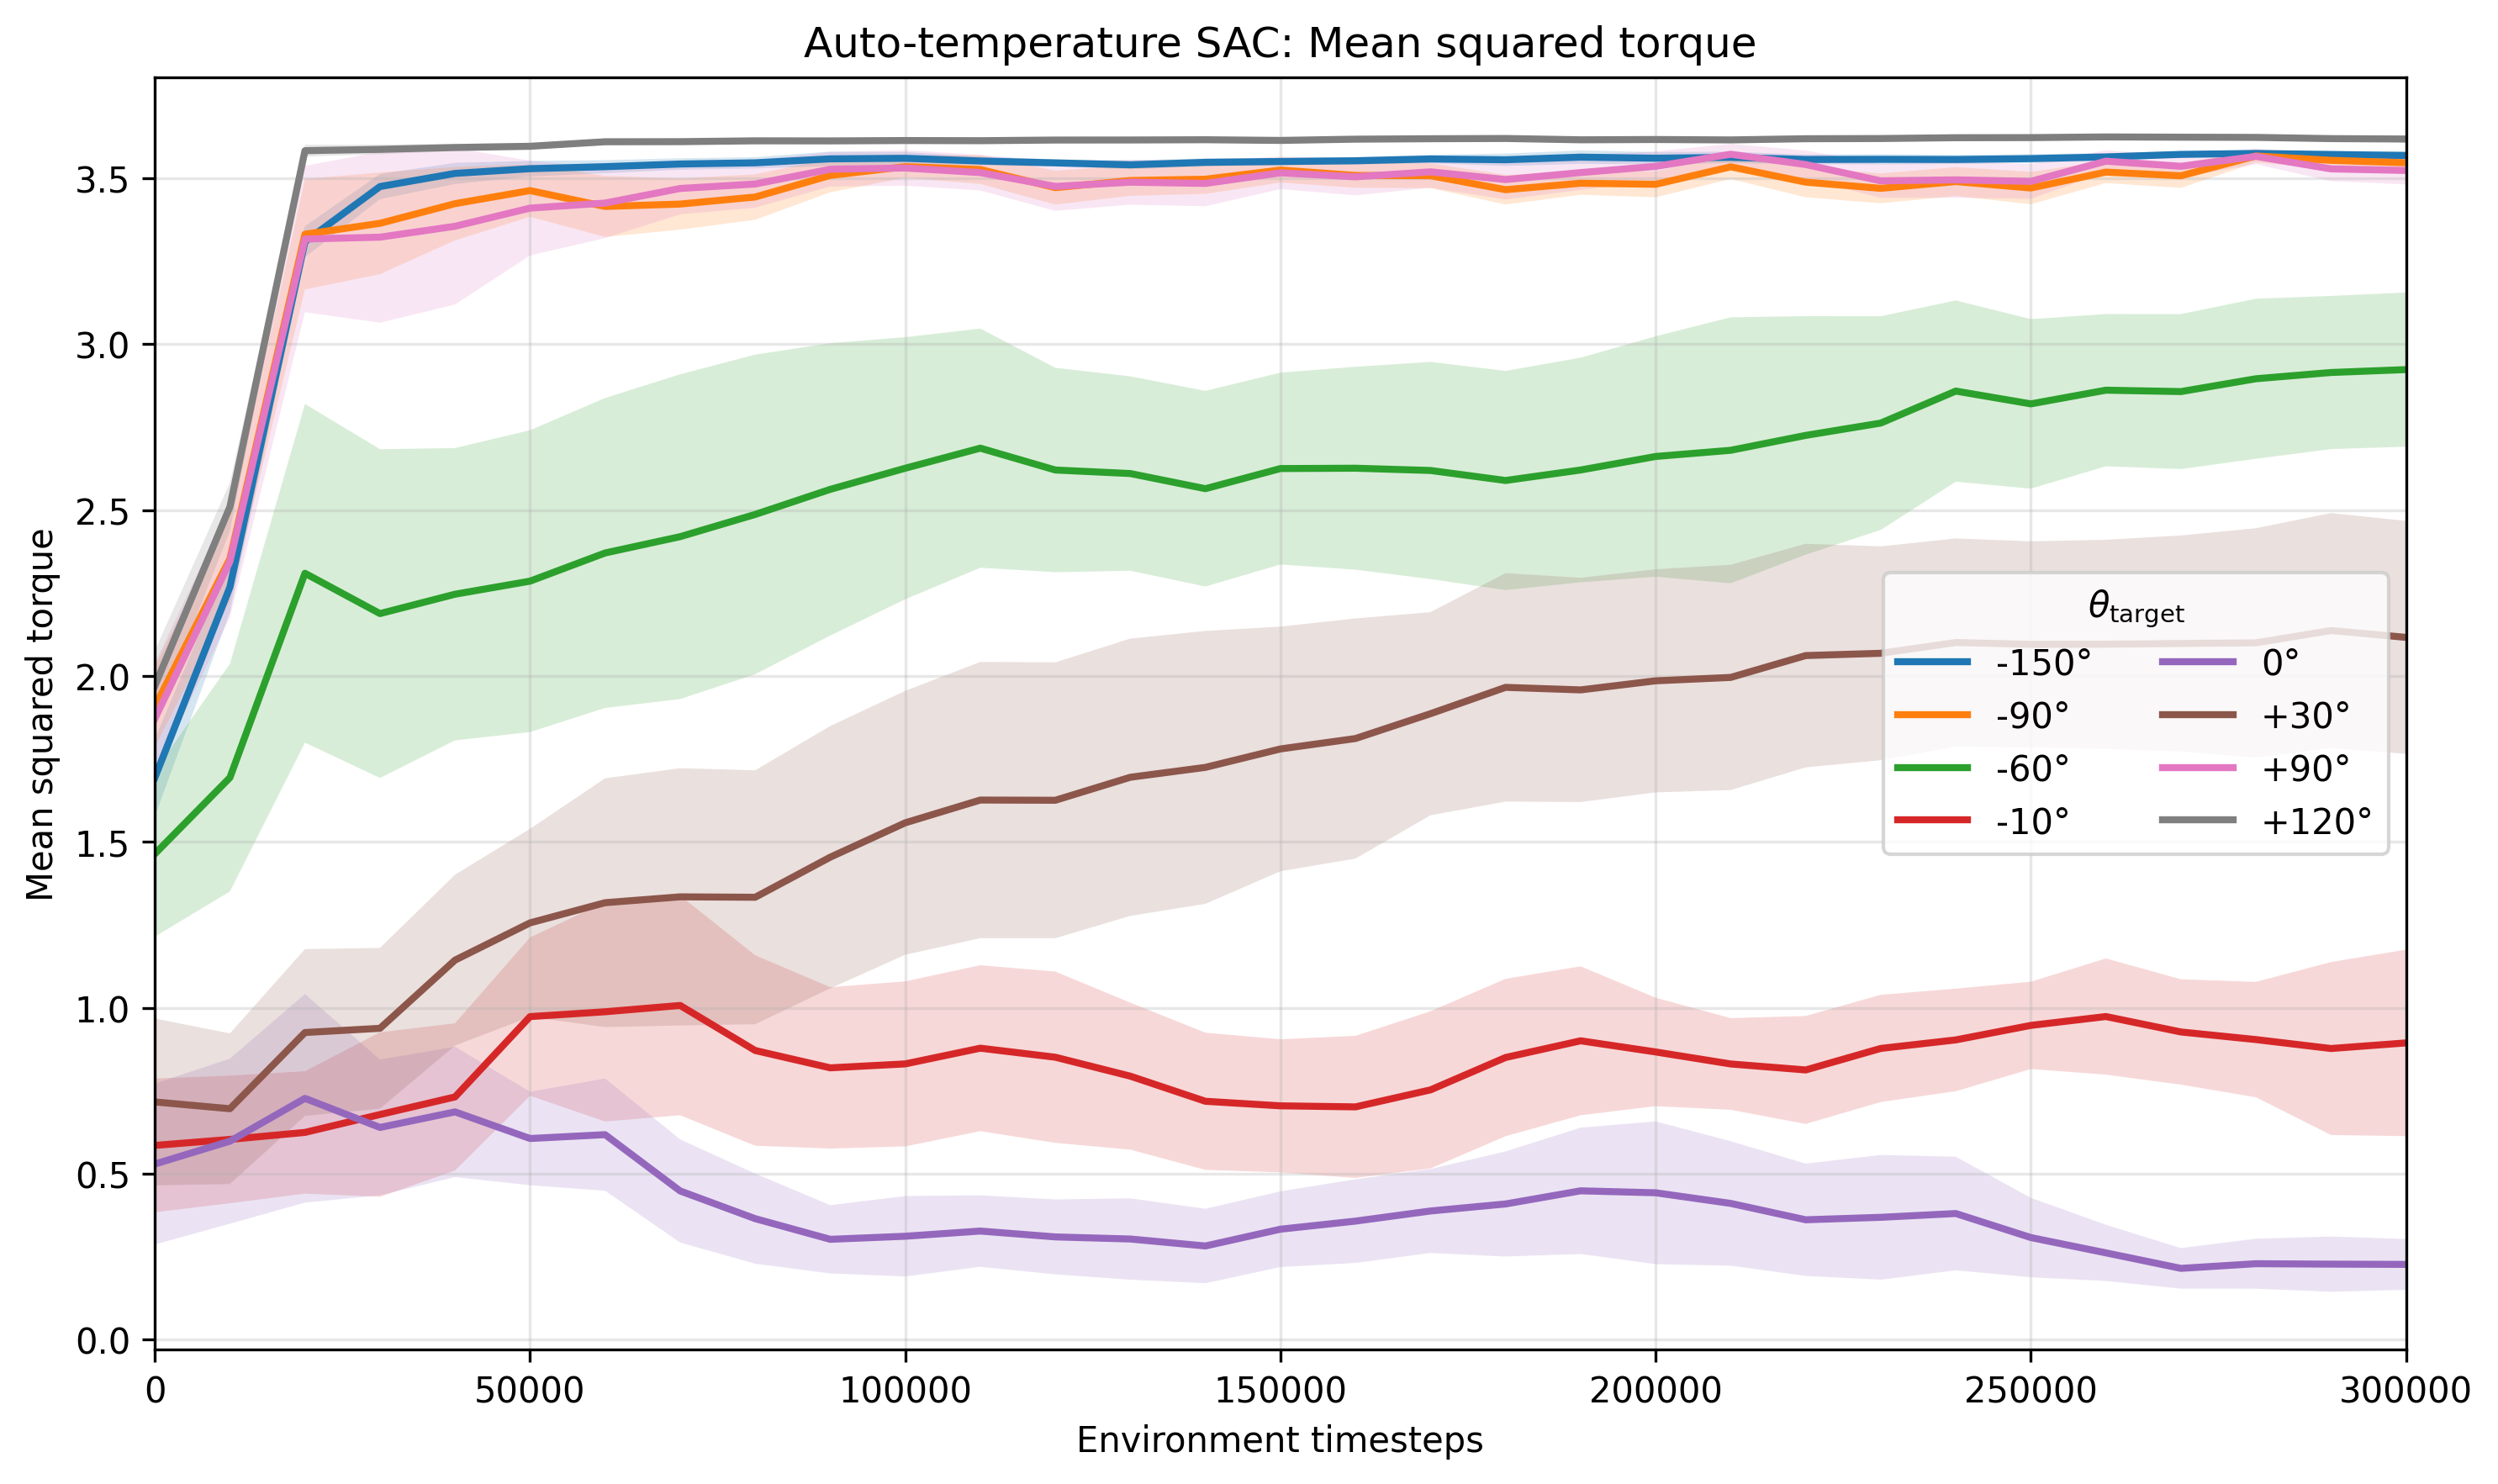
\includegraphics[width=\linewidth]{P1d_auto_all_targets_torque.png}
    \caption{Mean squared torque.}
\end{subfigure}
\caption{Behavior diagnostics for auto-$\alpha$ SAC across targets.}
\label{fig:pendulum_behavior_metrics}
\end{figure}

\section{Torque-Limit Diagnostic ($-60^\circ$)}
\label{app:torque_diag}

\begin{table}[H]
\centering
\caption{Effect of torque range on $\theta_{\text{target}}=-60^\circ$.}
\begin{tabular}{rrrrr}
\toprule
Setting & Final Return & Angle Error & Occupancy & Mean Sq.\ Torque \\
\midrule
Default $[-2,2]$ & $-903.54 \pm 368.75$ & $48.39^\circ$ & $0.002$ & $2.979$ \\
Wider $[-6,6]$ & $\approx -49$ & $\approx 2$--$3^\circ$ & $\approx 0.98$ & $\approx 18.7$ \\
\bottomrule
\end{tabular}
\end{table}

Holding at $-60^\circ$ requires $|u_{\text{hold}}| = 5|\sin(-60^\circ)| \approx 4.33$, which exceeds the default action limit $|u|\leq 2$. Exact static holding at $-60^\circ$ is therefore not feasible under the default torque range. With the wider range $[-6,6]$, the required holding torque becomes feasible and the policy achieves near-perfect tracking. This supports the torque-authority interpretation.

\begin{table}[H]
\centering
\caption{Static holding torque feasibility under default bound $|u|\leq 2$.}
\begin{tabular}{rrl}
\toprule
$\theta_{\text{target}}$ & $|u_{\text{hold}}| = 5|\sin\theta|$ & Feasible? \\
\midrule
$0^\circ$ & $0.00$ & Yes \\
$-10^\circ$ & $0.87$ & Yes \\
$30^\circ$ & $2.50$ & Borderline \\
$-60^\circ$ & $4.33$ & No \\
$90^\circ$ & $5.00$ & No \\
$-90^\circ$ & $5.00$ & No \\
$120^\circ$ & $4.33$ & No \\
$-150^\circ$ & $2.50$ & Borderline \\
\bottomrule
\end{tabular}
\end{table}

Borderline cases ($30^\circ$, $-150^\circ$) can still achieve good occupancy because the $10^\circ$ tolerance allows nearby angles requiring slightly lower holding torque, and dynamic regulation can keep the pendulum close to the target region.

\begin{figure}[H]
\centering
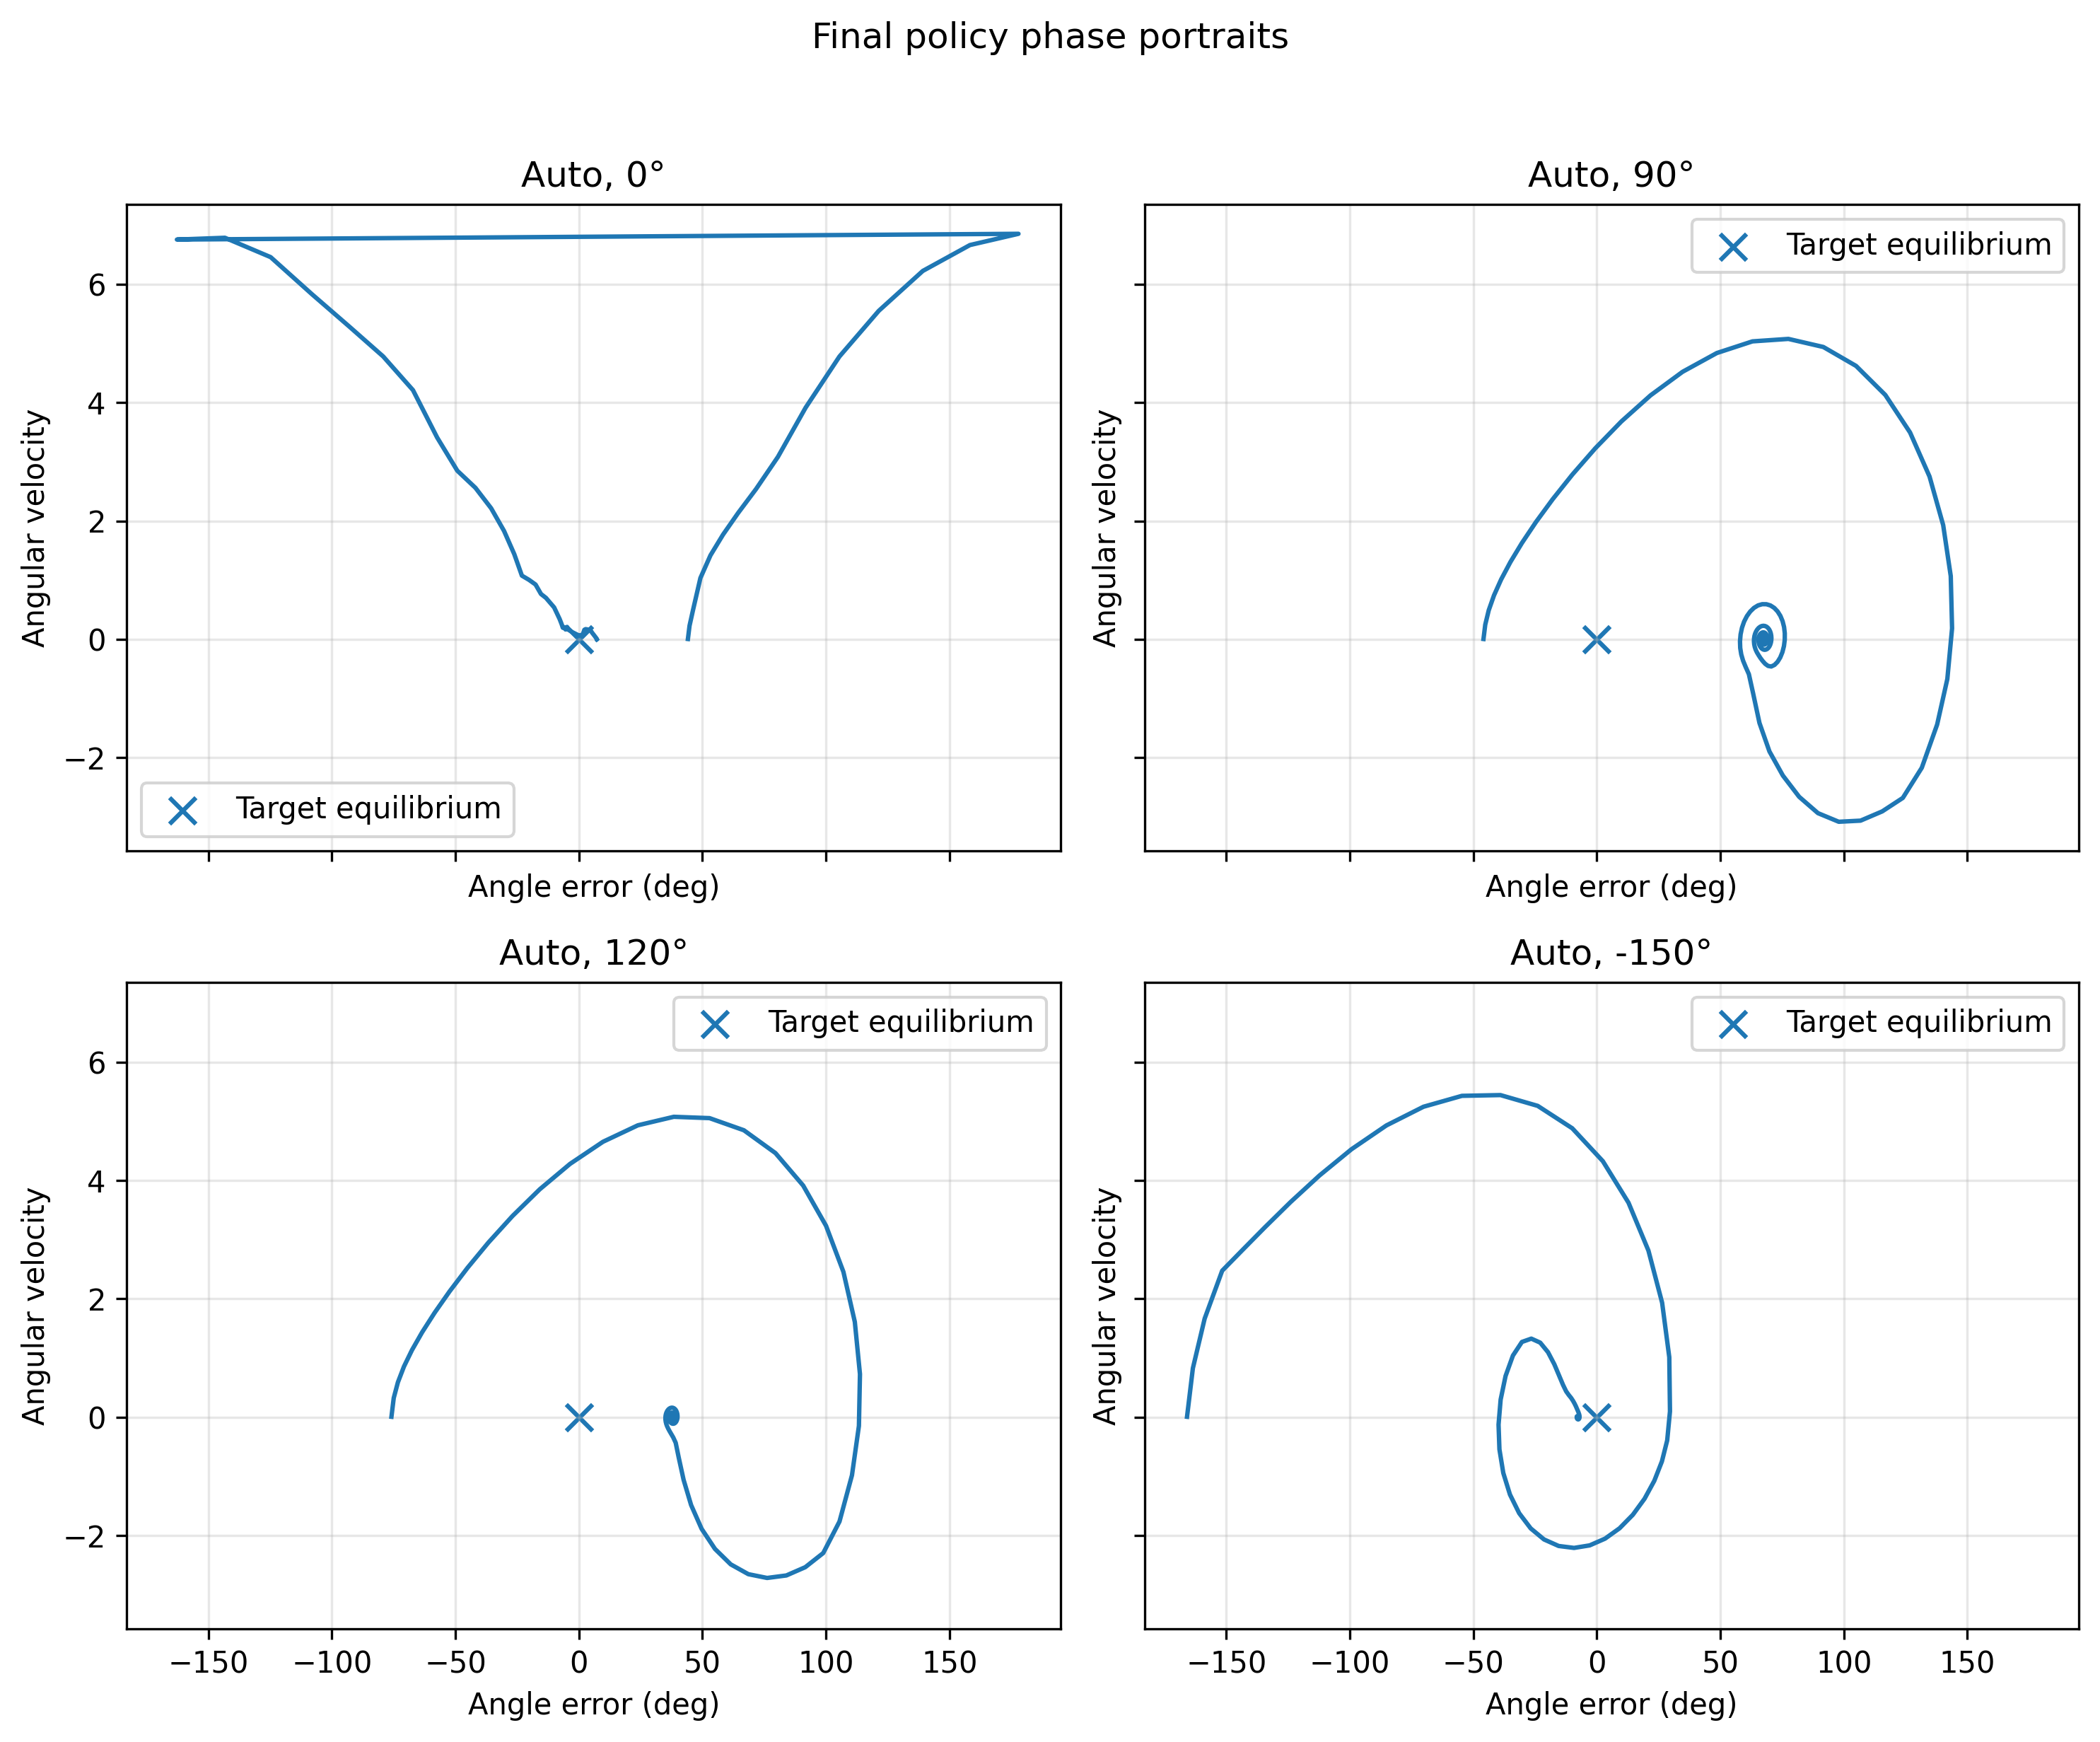
\includegraphics[width=0.72\textwidth]{A4_phase_portraits_selected_targets.png}
\caption{Phase portraits for selected final policies.}
\label{fig:pendulum_phase_portraits}
\end{figure}

\section{Additional Reacher Diagnostics}
\label{app:reacher_diag}

\begin{figure}[H]
    \centering
    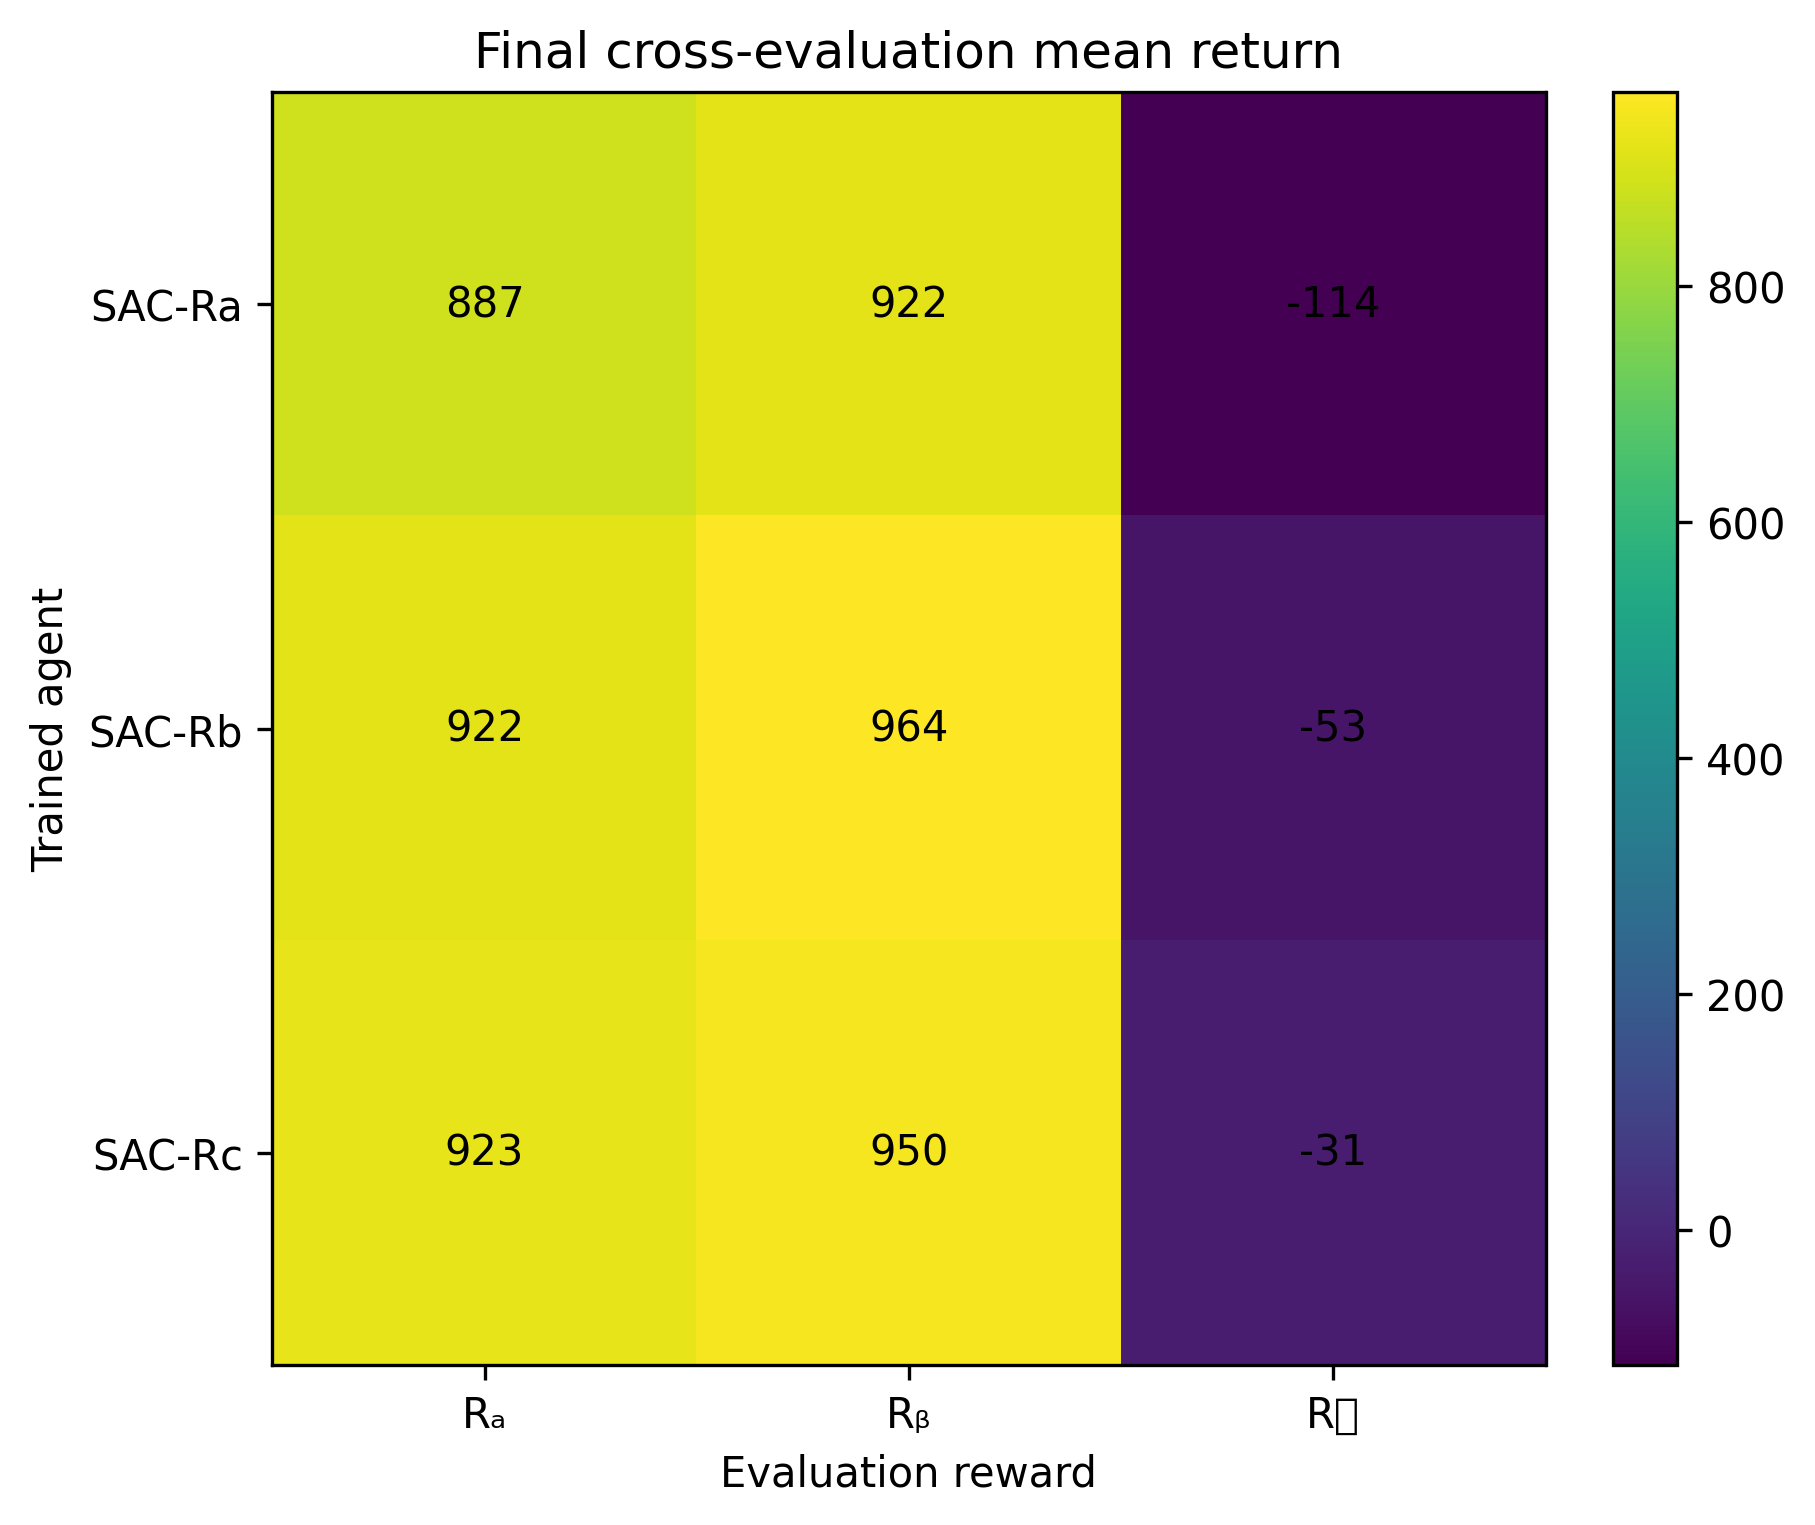
\includegraphics[width=0.68\textwidth]{reacher_final_return_heatmap.png}
    \caption{Final cross-evaluation mean returns for Reacher. Rows indicate the training reward and columns indicate the evaluation reward.}
    \label{fig:reacher-heatmap-appendix}
\end{figure}

The heatmap summarizes the final cross-evaluation point. All policies obtain high final returns under $R_a$ and $R_b$, showing that all three reward formulations learn target-reaching behavior. Under $R_c$, SAC-$R_c$ achieves the best value, confirming that the time-to-goal reward is most aligned with fast reaching.

\begin{figure}[H]
    \centering
    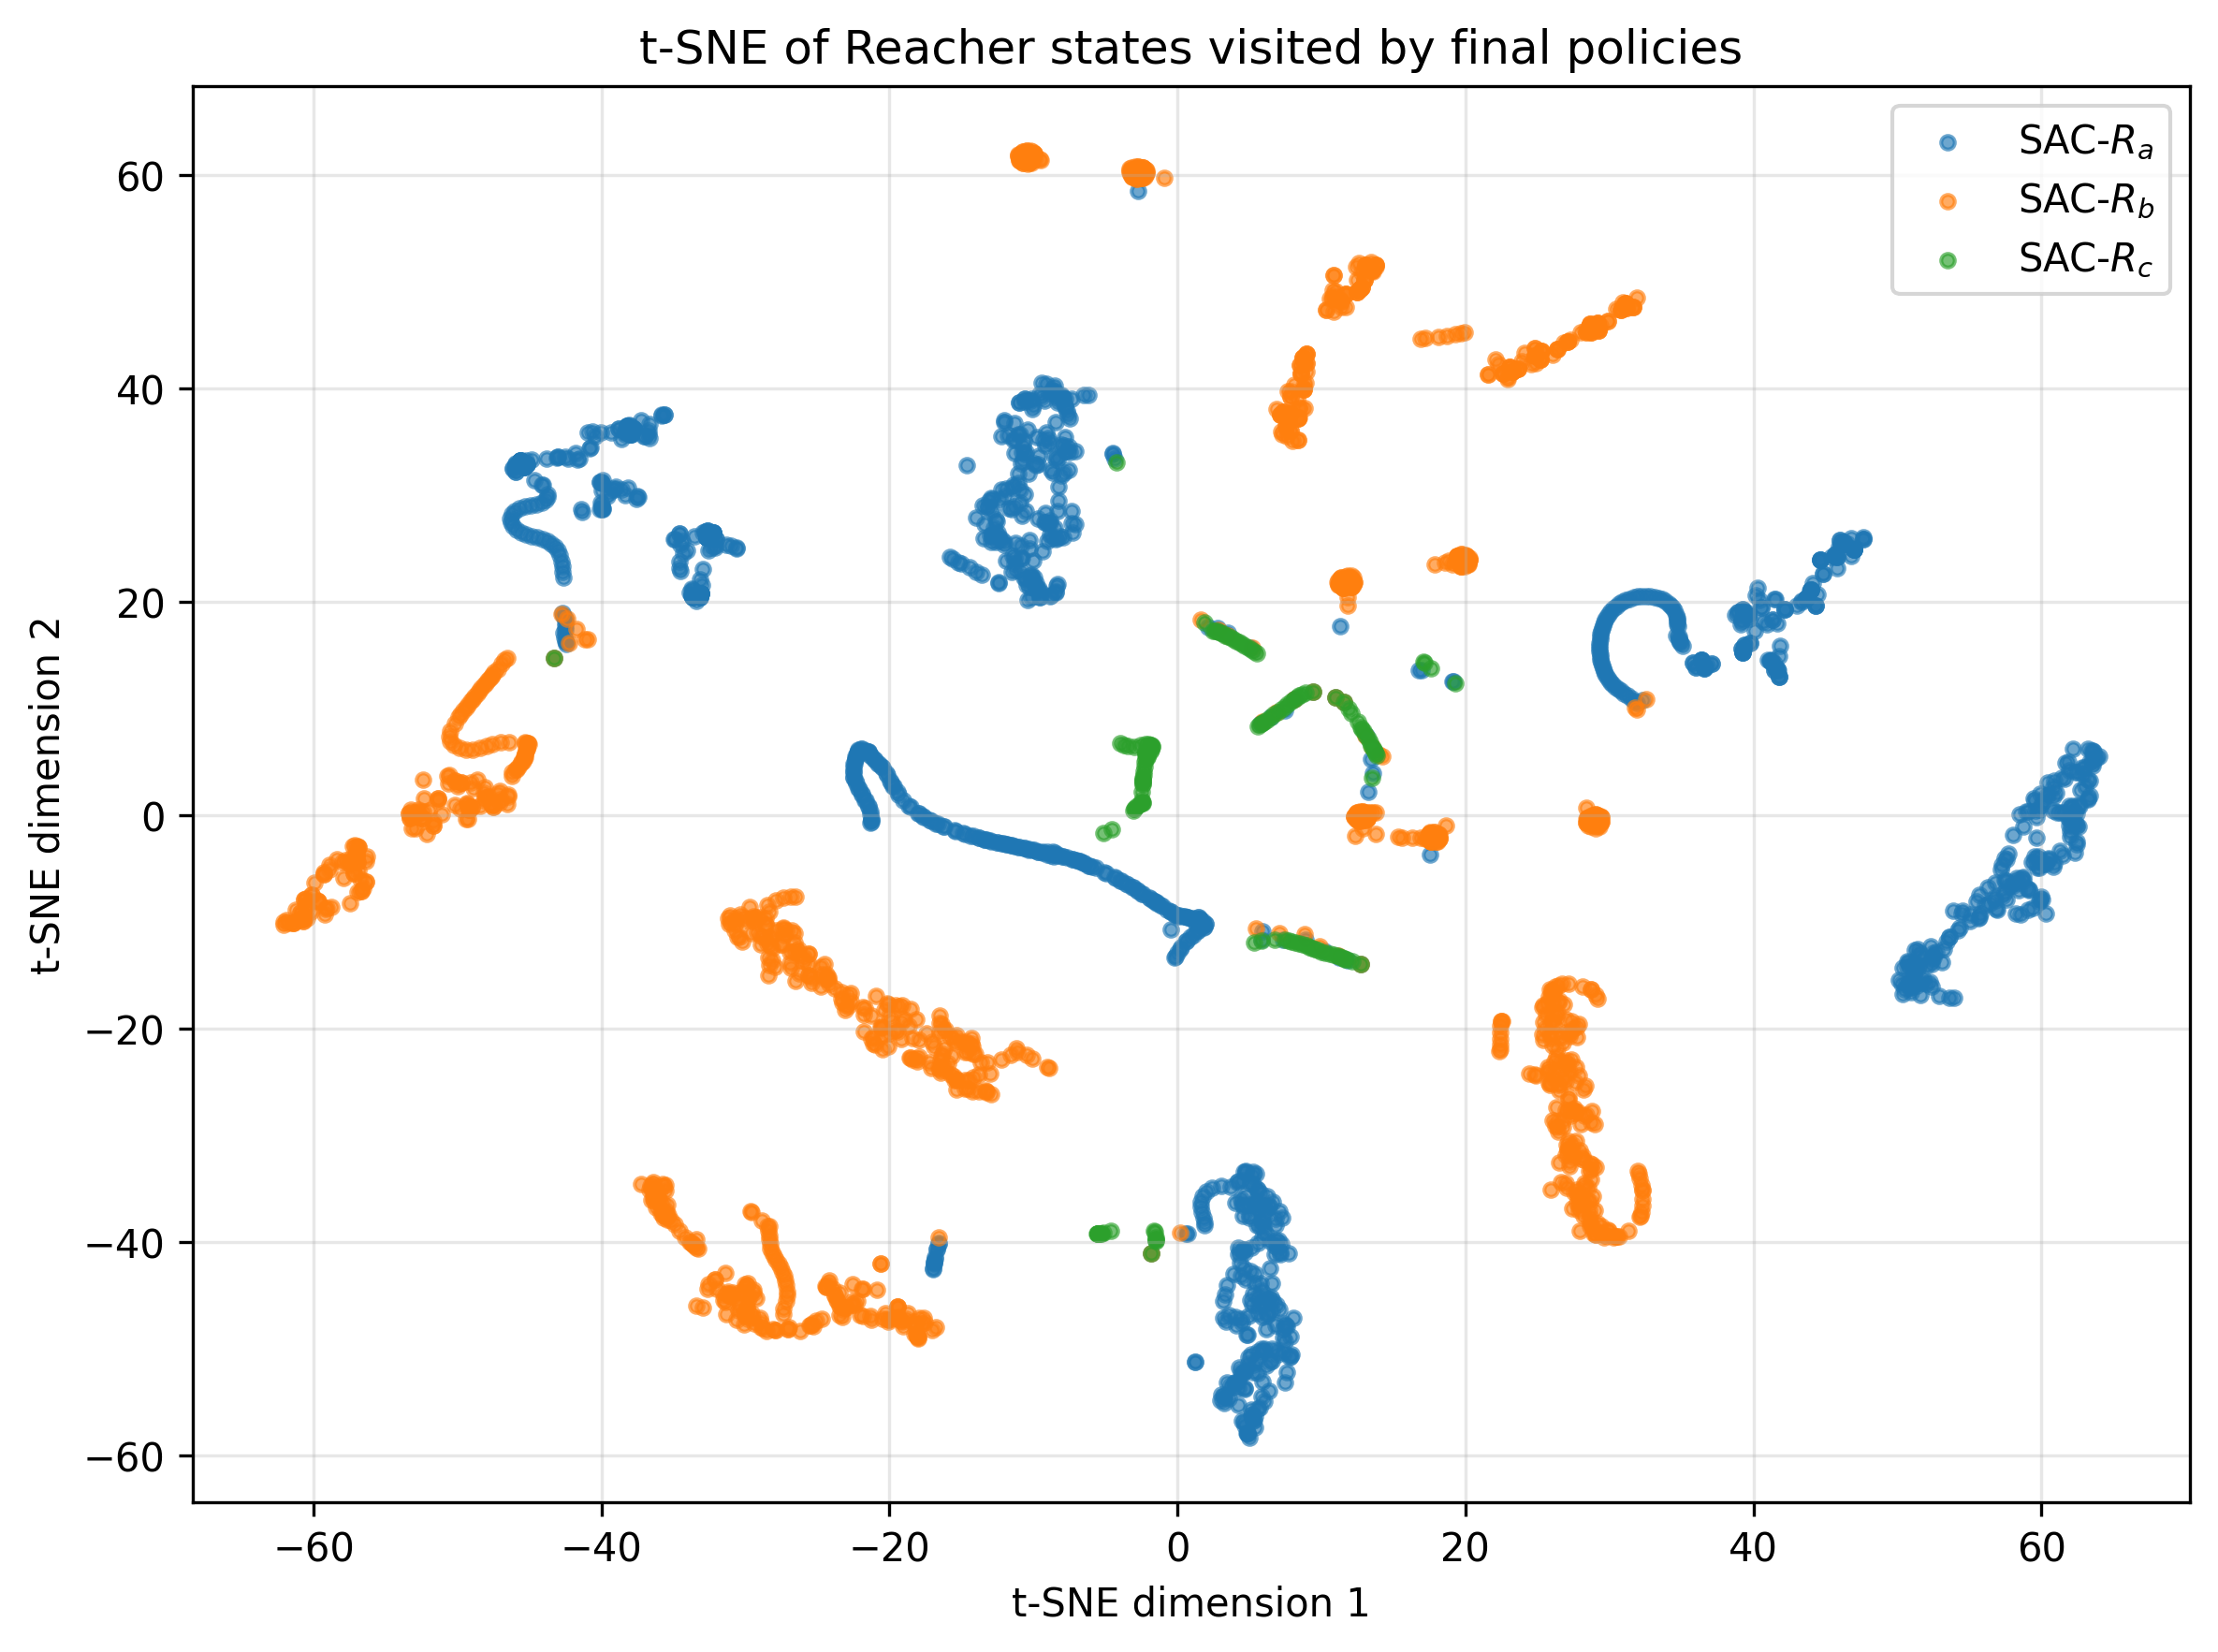
\includegraphics[width=0.68\textwidth]{reacher_tsne_by_policy.png}
    \caption{t-SNE projection of states visited by final Reacher policies. This visualization is qualitative only.}
    \label{fig:reacher-tsne-appendix}
\end{figure}

The t-SNE visualization shows that policies trained under different reward formulations visit different projected regions of the state space. This suggests that reward design affects trajectory distribution. Since t-SNE is only a nonlinear projection, we use it only as supporting qualitative evidence; the main conclusions are based on learning curves and final-policy behavioral metrics.

\begin{figure}[H]
    \centering
    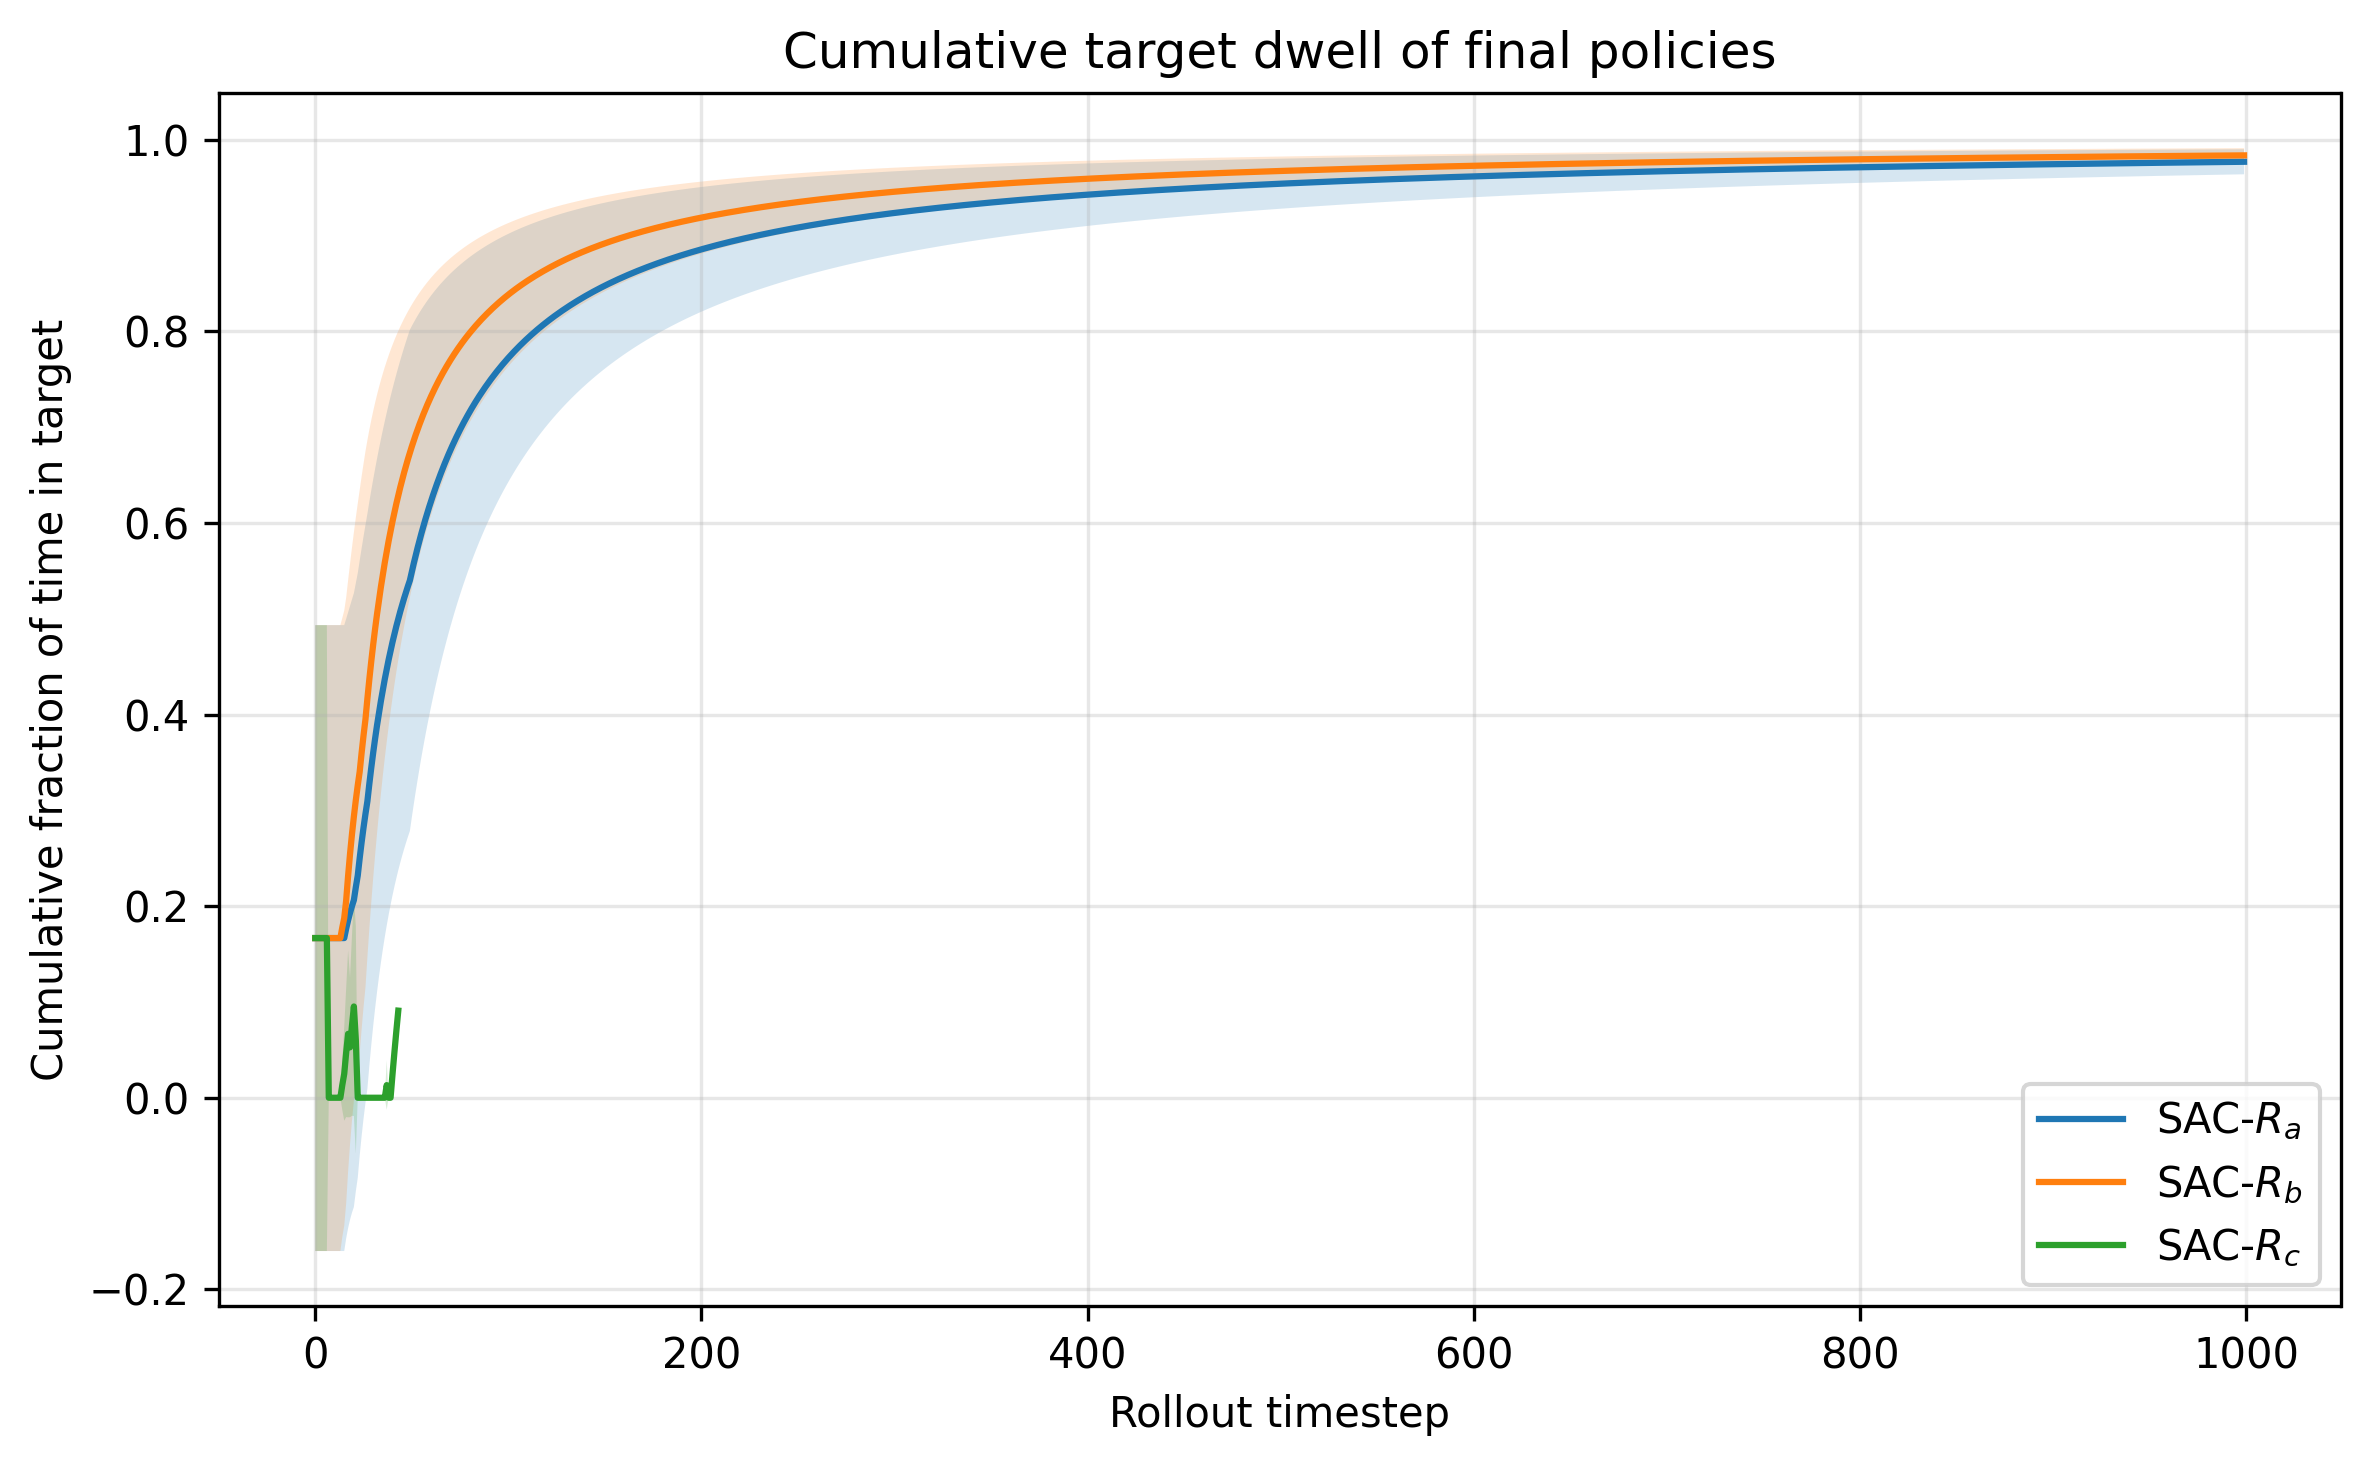
\includegraphics[width=0.68\textwidth]{reacher_cumulative_dwell_fraction.png}
    \caption{Cumulative fraction of rollout time spent inside the target. SAC-$R_c$ terminates early under its evaluation rule after reaching the target with low velocity, so its shorter curve indicates early success rather than poor dwell behavior.}
    \label{fig:reacher-dwell-appendix}
\end{figure}

The dwell plot shows that SAC-$R_a$ and SAC-$R_b$ quickly reach the target and spend most of the rollout inside it. SAC-$R_c$ is not directly comparable in this plot because the $R_c$ evaluation episode terminates once the target is reached with sufficiently low velocity. Therefore, the short SAC-$R_c$ curve should be interpreted as early successful termination.

\end{appendix}
\end{document}
